\documentclass[11pt]{article}

\usepackage[margin=1in]{geometry}
\usepackage{amsmath, amssymb, amsfonts}
\usepackage{booktabs}
\usepackage{array}
\usepackage{enumitem}
\usepackage{hyperref}
\usepackage{graphicx}
\usepackage{xcolor}

\hypersetup{
  colorlinks=true,
  linkcolor=blue,
  citecolor=blue,
  urlcolor=blue
}

\newcommand{\TODO}[1]{\textcolor{red}{[TODO: #1]}}
\newcommand{\sst}{\mathrm{SST}}
\newcommand{\tobs}{T_{\mathrm{land}}}
\newcommand{\twusd}{T^{\prime}_{\mathrm{WUSD}}}
\newcommand{\pc}[1]{\mathrm{PC}_{#1}}
\newcommand{\eof}[1]{\mathrm{EOF}_{#1}}
\newcommand{\evr}{\mathrm{EVR}}

\title{Current Status: SST Principal Components and Overland Temperature Response}
\author{Template Research Note}
\date{\today}

\begin{document}
\maketitle


\section{Observed SST and T2m Response Structure}
\label{sec:observed}

This section defines the observational relationship between large-scale SST variability and
observed overland near-surface air temperature. Both the SST field and the T2m response field
are treated here as observation-based reference datasets. The current workflow uses leading COBE2
SST modes as a reduced predictor basis and evaluates how much observed ERA5-Land T2m variability
can be explained by those modes.

\subsection{Data Sources and Notation}
\label{subsec:data_notation}

The current observational workflow uses the following source datasets and derived fields:
\begin{itemize}[leftmargin=1.5em]
  \item COBE2 monthly SST source:
  \texttt{/global/cfs/projectdirs/m3522/datalake/COBE2/sst.mon.mean.nc}
  \item ERA5-Land monthly mean T2m artifact:
  \texttt{/pscratch/sd/h/hyvchen/Snow-Predication-at-Sierra/artifacts/era5land\_t2m\_monthly\_anomalies/era5land\_t2m\_monthly\_mean.nc}
  \item ERA5-Land monthly climatology artifact:
  \texttt{/pscratch/sd/h/hyvchen/Snow-Predication-at-Sierra/artifacts/era5land\_t2m\_monthly\_anomalies/era5land\_t2m\_monthly\_climatology.nc}
\end{itemize}

\begin{table}[h]
\centering
\begin{tabular}{>{\raggedright\arraybackslash}p{0.20\linewidth} >{\raggedright\arraybackslash}p{0.72\linewidth}}
\toprule
Symbol & Meaning \\
\midrule
$x$ & SST grid location on the COBE2 EOF grid. \\
$r$ & Overland T2m grid location. \\
$t$ & Monthly time index. \\
$m(t)$ & Calendar month corresponding to time $t$. \\
$K$ & Number of retained SST modes; current default target is $K=6$. \\
$\sst(x,t)$ & Raw monthly sea surface temperature field. \\
$\sst^{\prime}(x,t)$ & SST anomaly after monthly climatology removal. \\
$\pc{k}(t)$ & Observed COBE2 principal component time series for mode $k$. \\
$\eof{k}(x)$ & COBE2 EOF loading pattern for mode $k$. \\
$\tobs(r,t)$ & Observed overland T2m anomaly, typically ERA5-Land based. \\
$\twusd(r,t)$ & WUSD-03 overland T2m anomaly. \\
$\beta_k(r)$ & Observed T2m sensitivity to SST mode $k$. \\
$\widetilde{\beta}_k(r)$ & WUSD-03 T2m sensitivity to projected SST mode $k$. \\
\bottomrule
\end{tabular}
\caption{Compact notation used in the SST--T2m response analysis.}
\label{tab:notation}
\end{table}

\subsection{SST Anomalies and EOF Decomposition}
\label{subsec:sst_eof}

We begin with monthly COBE2 SST and remove the monthly climatology to isolate anomalies:
\begin{equation}
\sst^{\prime}(x,t) = \sst(x,t) - \overline{\sst}_{m(t)}(x),
\label{eq:sst_anomaly}
\end{equation}
where $\overline{\sst}_{m}(x)$ is the climatological mean SST at location $x$ for calendar month $m$.
Here ``monthly climatology'' means a month-of-year mean computed across all available years at each
grid cell. For example, the February anomaly at location $x$ is formed by taking the SST in a given
February and subtracting the mean of all February SST values at that same location across the full
record. The same month-specific subtraction is applied separately for January, March, and the other
calendar months.

The anomaly field is then reshaped into a time--space matrix prior to EOF analysis.
The current EOF preprocessing choices are summarized in Table~\ref{tab:eof_preprocessing}.

\begin{table}[h]
\centering
\begin{tabular}{>{\raggedright\arraybackslash}p{0.26\linewidth} >{\raggedright\arraybackslash}p{0.66\linewidth}}
\toprule
Item & Current implementation \\
\midrule
Reshaping &
The anomaly cube is reshaped from $(\mathrm{time},\mathrm{lat},\mathrm{lon})$ to
$A(\mathrm{time},\mathrm{space})$ by flattening the latitude--longitude dimensions into one spatial axis. \\
Spatial mask &
After reshaping, the EOF solve keeps only SST grid cells that are finite at every monthly time step:
\texttt{np.isfinite(anomalies\_flat).all(axis=0)}. Missing-value and land points are first converted to
\texttt{NaN}, so the retained columns are all-time-finite ocean cells within the chosen domain. \\
Latitude weighting &
Each retained spatial column is multiplied by $\sqrt{\cos(\mathrm{lat})}$ before the EOF solve, so the
variance metric is area weighted. \\
Saved EOF units &
The EOF solve is performed on the weighted matrix, but the saved EOF maps are converted back to
unweighted SST-loading units by dividing each retained column by the same
$\sqrt{\cos(\mathrm{lat})}$ factor after the solve. \\
Standardization &
No additional per-grid-cell standardization is applied after anomaly construction. There is no local
z-scoring, no unit-variance rescaling of columns, and no extra temporal detrending in this EOF step. \\
PC scaling &
The principal components are the raw leading SVD amplitudes of the weighted anomaly matrix. Any later
normalization should be documented explicitly in the downstream regression or projection analysis. \\
Code paths &
Regional workflow:
\texttt{scripts/compute\_cobe2\_pacific\_sierra\_pc\_era5\_t2m\_patterns.py}. Global reference:
\texttt{scripts/run\_cobe2\_global\_sst\_eof\_reproduction.py}. Shared anomaly helper:
\texttt{scripts/run\_sst\_monthly\_climatology\_eof\_diagnostics.py}. \\
\bottomrule
\end{tabular}
\caption{Code-backed summary of the current SST EOF preprocessing pipeline.}
\label{tab:eof_preprocessing}
\end{table}

The current scientific intent is to preserve the dominant SST covariance structure while reducing the
predictor dimension from a full field to a small set of leading modes.

The conceptual EOF/PCA approximation is
\begin{equation}
\sst^{\prime}(x,t) \approx \sum_{k=1}^{K} \pc{k}(t)\,\eof{k}(x),
\label{eq:eof_expansion}
\end{equation}
with $K=6$ retained for the current teleconnection analysis.

\paragraph{Why use PCs.}
SST is high dimensional in space, and direct regression from every ocean grid cell to land T2m is
not the current target representation. The leading PCs provide a compact basis for dominant SST
variability, reduce collinearity among predictors, and make the downstream SST--T2m response maps
easier to compare across observations and model output.

% TODO: Add figure showing EOF1--EOF6 spatial patterns and PC1--PC6 time series.
% Suggested figure: COBE2 EOF/PC summary plot.

\subsection{Regression from SST PCs to Overland T2m}
\label{subsec:obs_regression}

Observed overland T2m anomalies are represented as a response to the retained SST PCs:
\begin{equation}
\tobs(r,t) = \sum_{k=1}^{K} \beta_k(r)\,\pc{k}(t) + \epsilon(r,t),
\label{eq:obs_regression}
\end{equation}
where $\epsilon(r,t)$ collects variance not explained by the retained SST basis.

In the current observational workflow, this is treated as a standard vector projection problem at
each land grid point $r$: we approximate the local ERA5-Land anomaly time series using the direction
of SST PC $k$. Writing $Y(t,r)$ for the ERA5-Land T2m anomaly and $a_k(t)$ for COBE2 SST PC $k$,
the projection coefficient is
\begin{equation}
\beta_k(r) = \frac{a_k^\top Y(:,r)}{a_k^\top a_k}
= \frac{\sum_t a_k(t)\,Y(t,r)}{\sum_t a_k(t)^2}.
\label{eq:beta_projection}
\end{equation}
This is the best one-coefficient projection of the local T2m anomaly vector onto the direction of
PC $k$. In the current code path, both the COBE2 SST field and the ERA5-Land T2m field are subset
to the same Pacific analysis region before the diagnostic is computed:
latitude $-10^\circ$ to $60^\circ$ and longitude $120^\circ$ to $280^\circ$ in $0..360$
coordinates. The implementation for the level-1 observed diagnostic is
\texttt{scripts/run\_cobe2\_pacific\_sierra\_t2m\_level1\_diagnostic.py}. In that script, the COBE2
PC matrix is always standardized over the overlap months using the sample mean and sample standard
deviation (\texttt{ddof=1}), so the response coefficient is interpreted as kelvin per
one-standard-deviation increase in PC $k$. The implemented pattern is therefore a standardized-PC,
projection-style ERA5-Land anomaly map,
\begin{equation}
\beta_k(r) \propto \frac{\sum_t \pc{k}(t)\,T_{\mathrm{land}}(r,t)}{\mathrm{std}(\pc{k})},
\label{eq:beta_weighted_pattern}
\end{equation}
computed from the native ERA5-Land monthly anomaly field built from the monthly mean and monthly
climatology artifacts after the same Pacific-region subsetting. The same source script also computes
the correlation map
\begin{equation}
\rho_k(r) = \mathrm{corr}\!\left(a_k(t), Y(t,r)\right),
\label{eq:rho_projection}
\end{equation}
and the local explained-variance map
\begin{equation}
R_k^2(r) = \rho_k(r)^2.
\label{eq:r2_projection}
\end{equation}
These three outputs, $\beta_k(r)$, $\rho_k(r)$, and $R_k^2(r)$, form the current single-PC
observational response diagnostic.

\begin{table}[h]
\centering
\begin{tabular}{>{\raggedright\arraybackslash}p{0.20\linewidth} >{\raggedright\arraybackslash}p{0.25\linewidth} >{\raggedright\arraybackslash}p{0.45\linewidth}}
\toprule
Quantity & Meaning & Interpretation \\
\midrule
$\beta_k(r)$ &
Local T2m response coefficient for PC $k$. &
Because the PCs are standardized in the level-1 script, $\beta_k(r)$ is read as kelvin change in
local ERA5-Land T2m anomaly per one-standard-deviation increase in PC $k$. Positive values indicate
warmer land anomalies when PC $k$ is positive; negative values indicate cooler anomalies. \\
$\rho_k(r)$ &
Temporal correlation between PC $k$ and local T2m anomaly. &
This measures the strength and sign of the linear co-variability. Values near $+1$ mean the local
T2m anomaly rises and falls with PC $k$, values near $-1$ mean the response is opposite in sign,
and values near $0$ mean little linear relationship. \\
$R_k^2(r)$ &
Single-PC local explained-variance fraction. &
This is the fraction of local T2m variance explained by perfect knowledge of SST PC $k$ alone in
the current single-PC diagnostic. Since $R_k^2(r)=\rho_k(r)^2$, it is always nonnegative and does
not preserve the response sign. \\
Source script &
Level-1 observed diagnostic implementation. &
\texttt{scripts/run\_cobe2\_pacific\_sierra\_t2m\_level1\_diagnostic.py} computes the standardized
PCs, $\beta_k(r)$ maps, $\rho_k(r)$ maps, and $R_k^2(r)$ maps together. \\
\bottomrule
\end{tabular}
\caption{Summary of the current single-PC observed SST--T2m response diagnostics.}
\label{tab:level1_diagnostic_summary}
\end{table}

\begin{figure}[h]
\centering
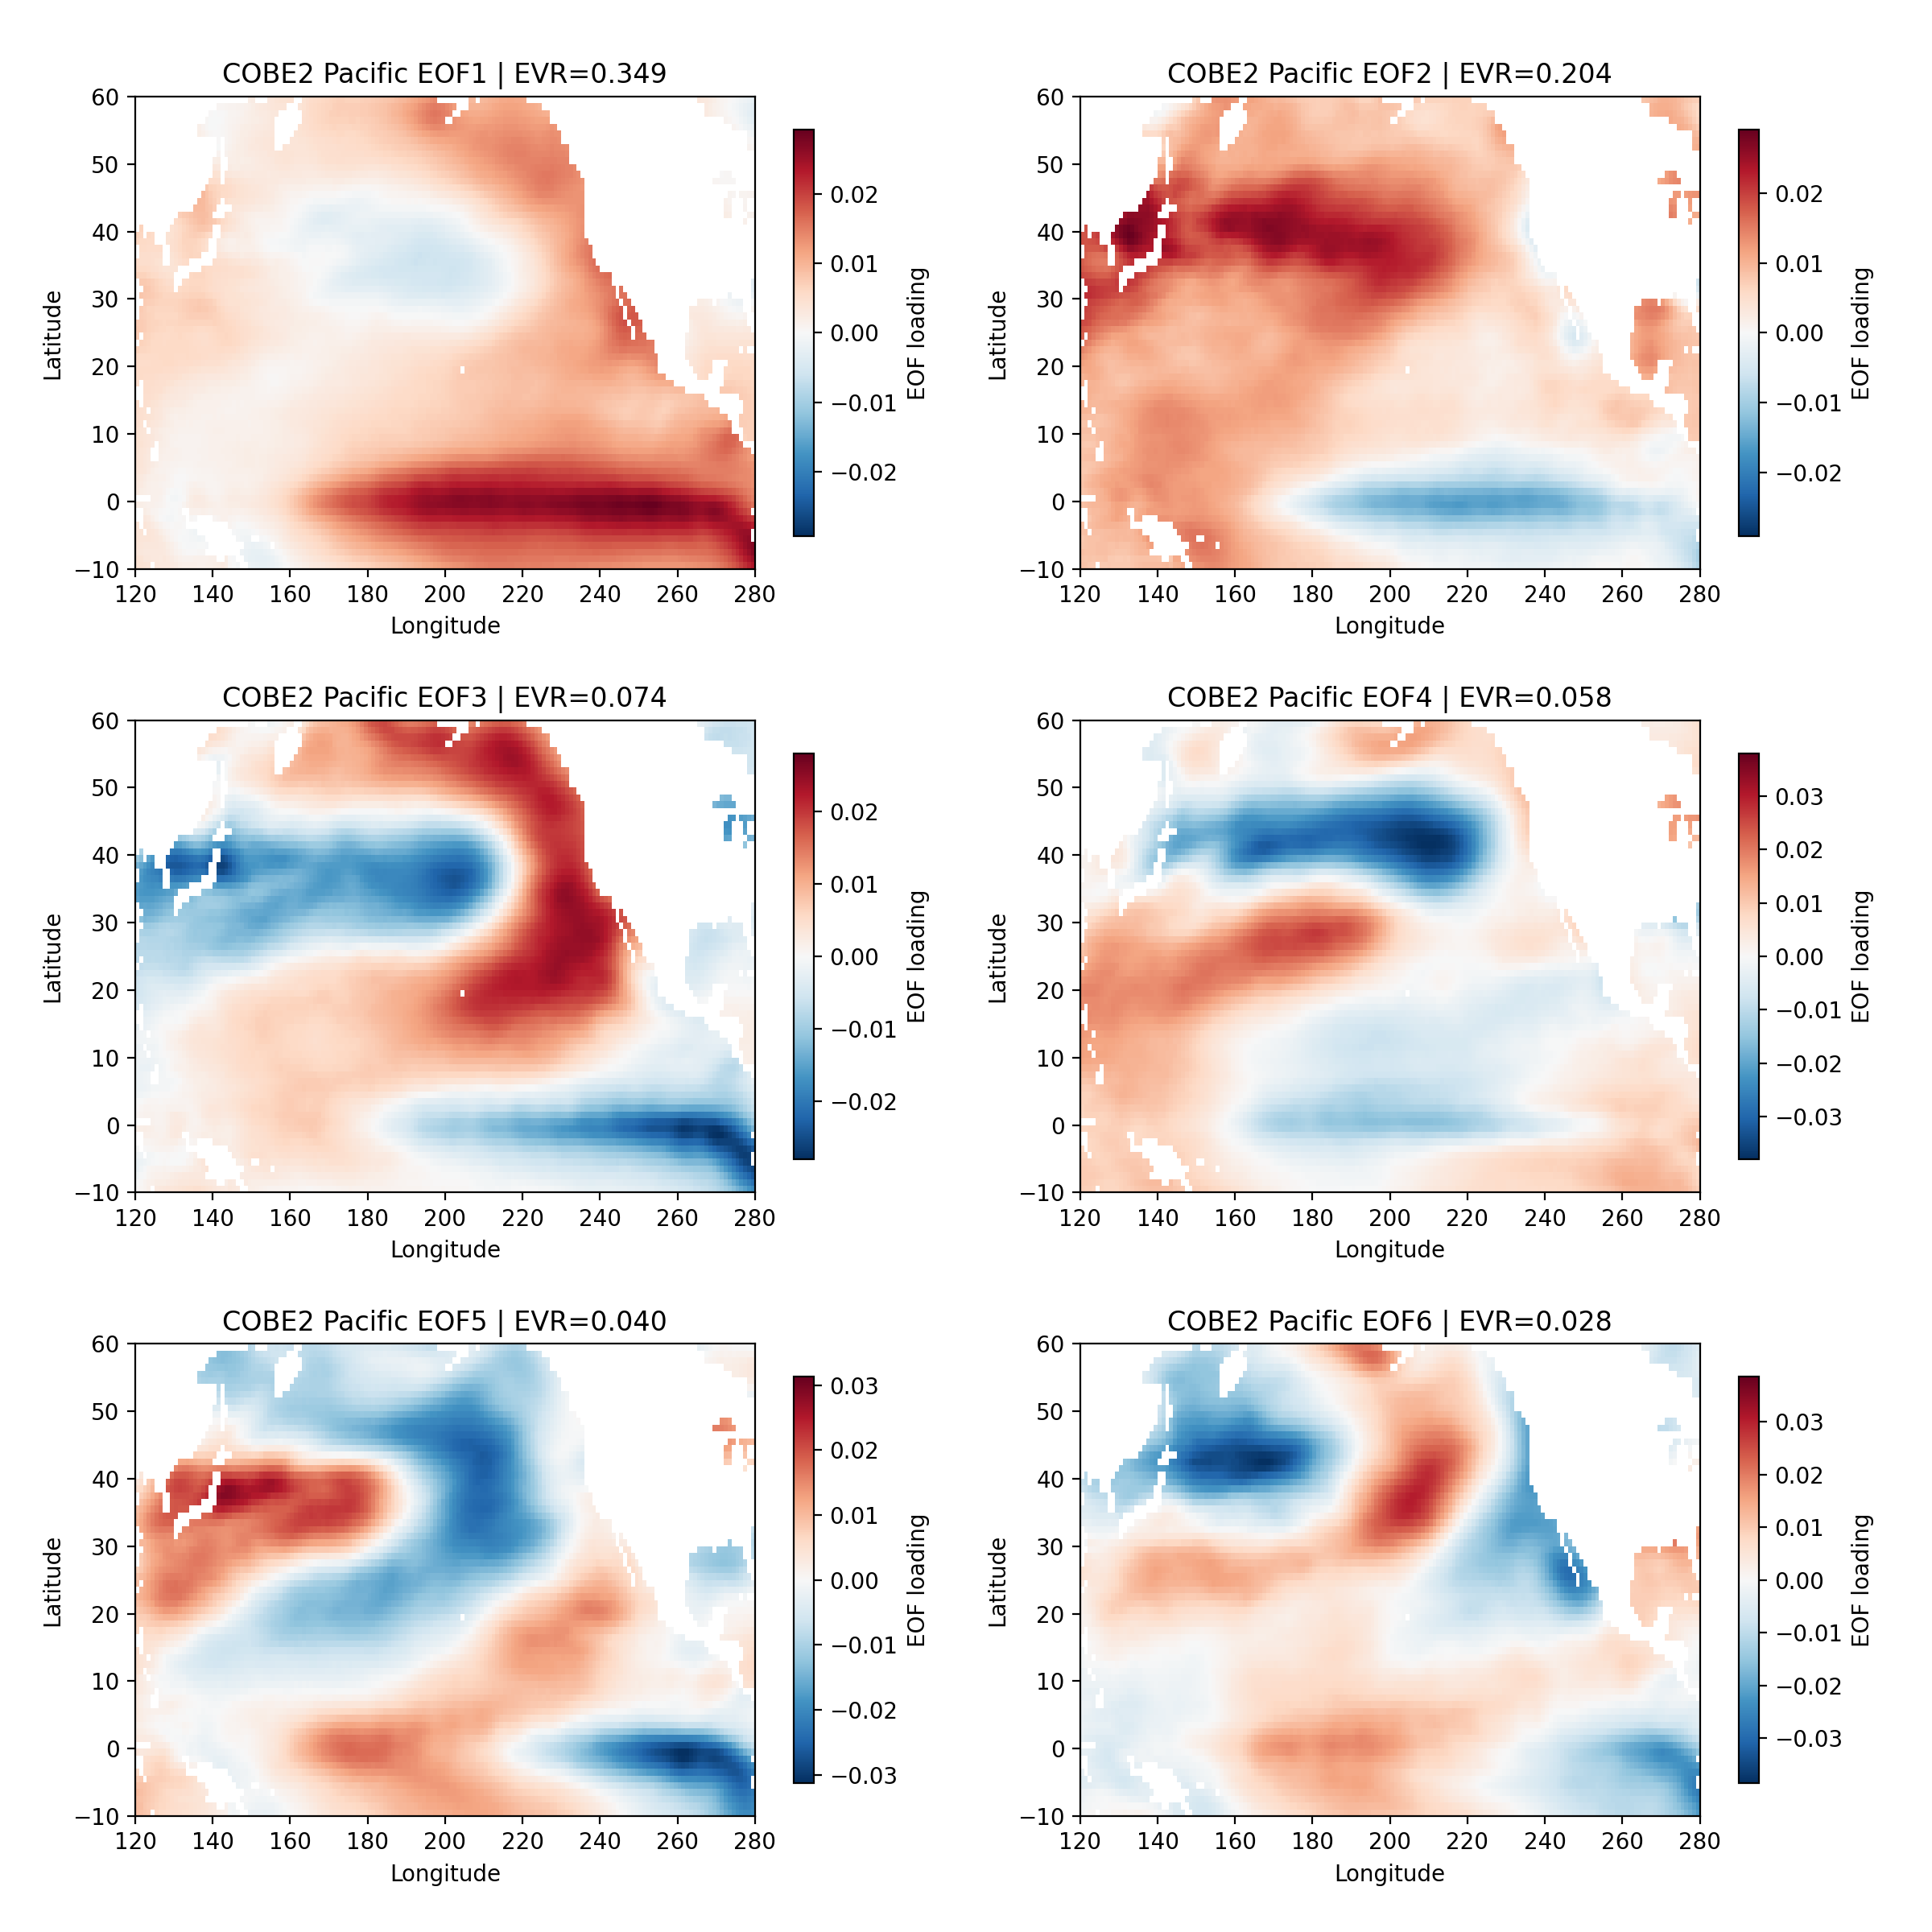
\includegraphics[width=0.49\linewidth]{../figures/cobe2_pacific_sierra_cobe2_eofs_modes1to6.png}
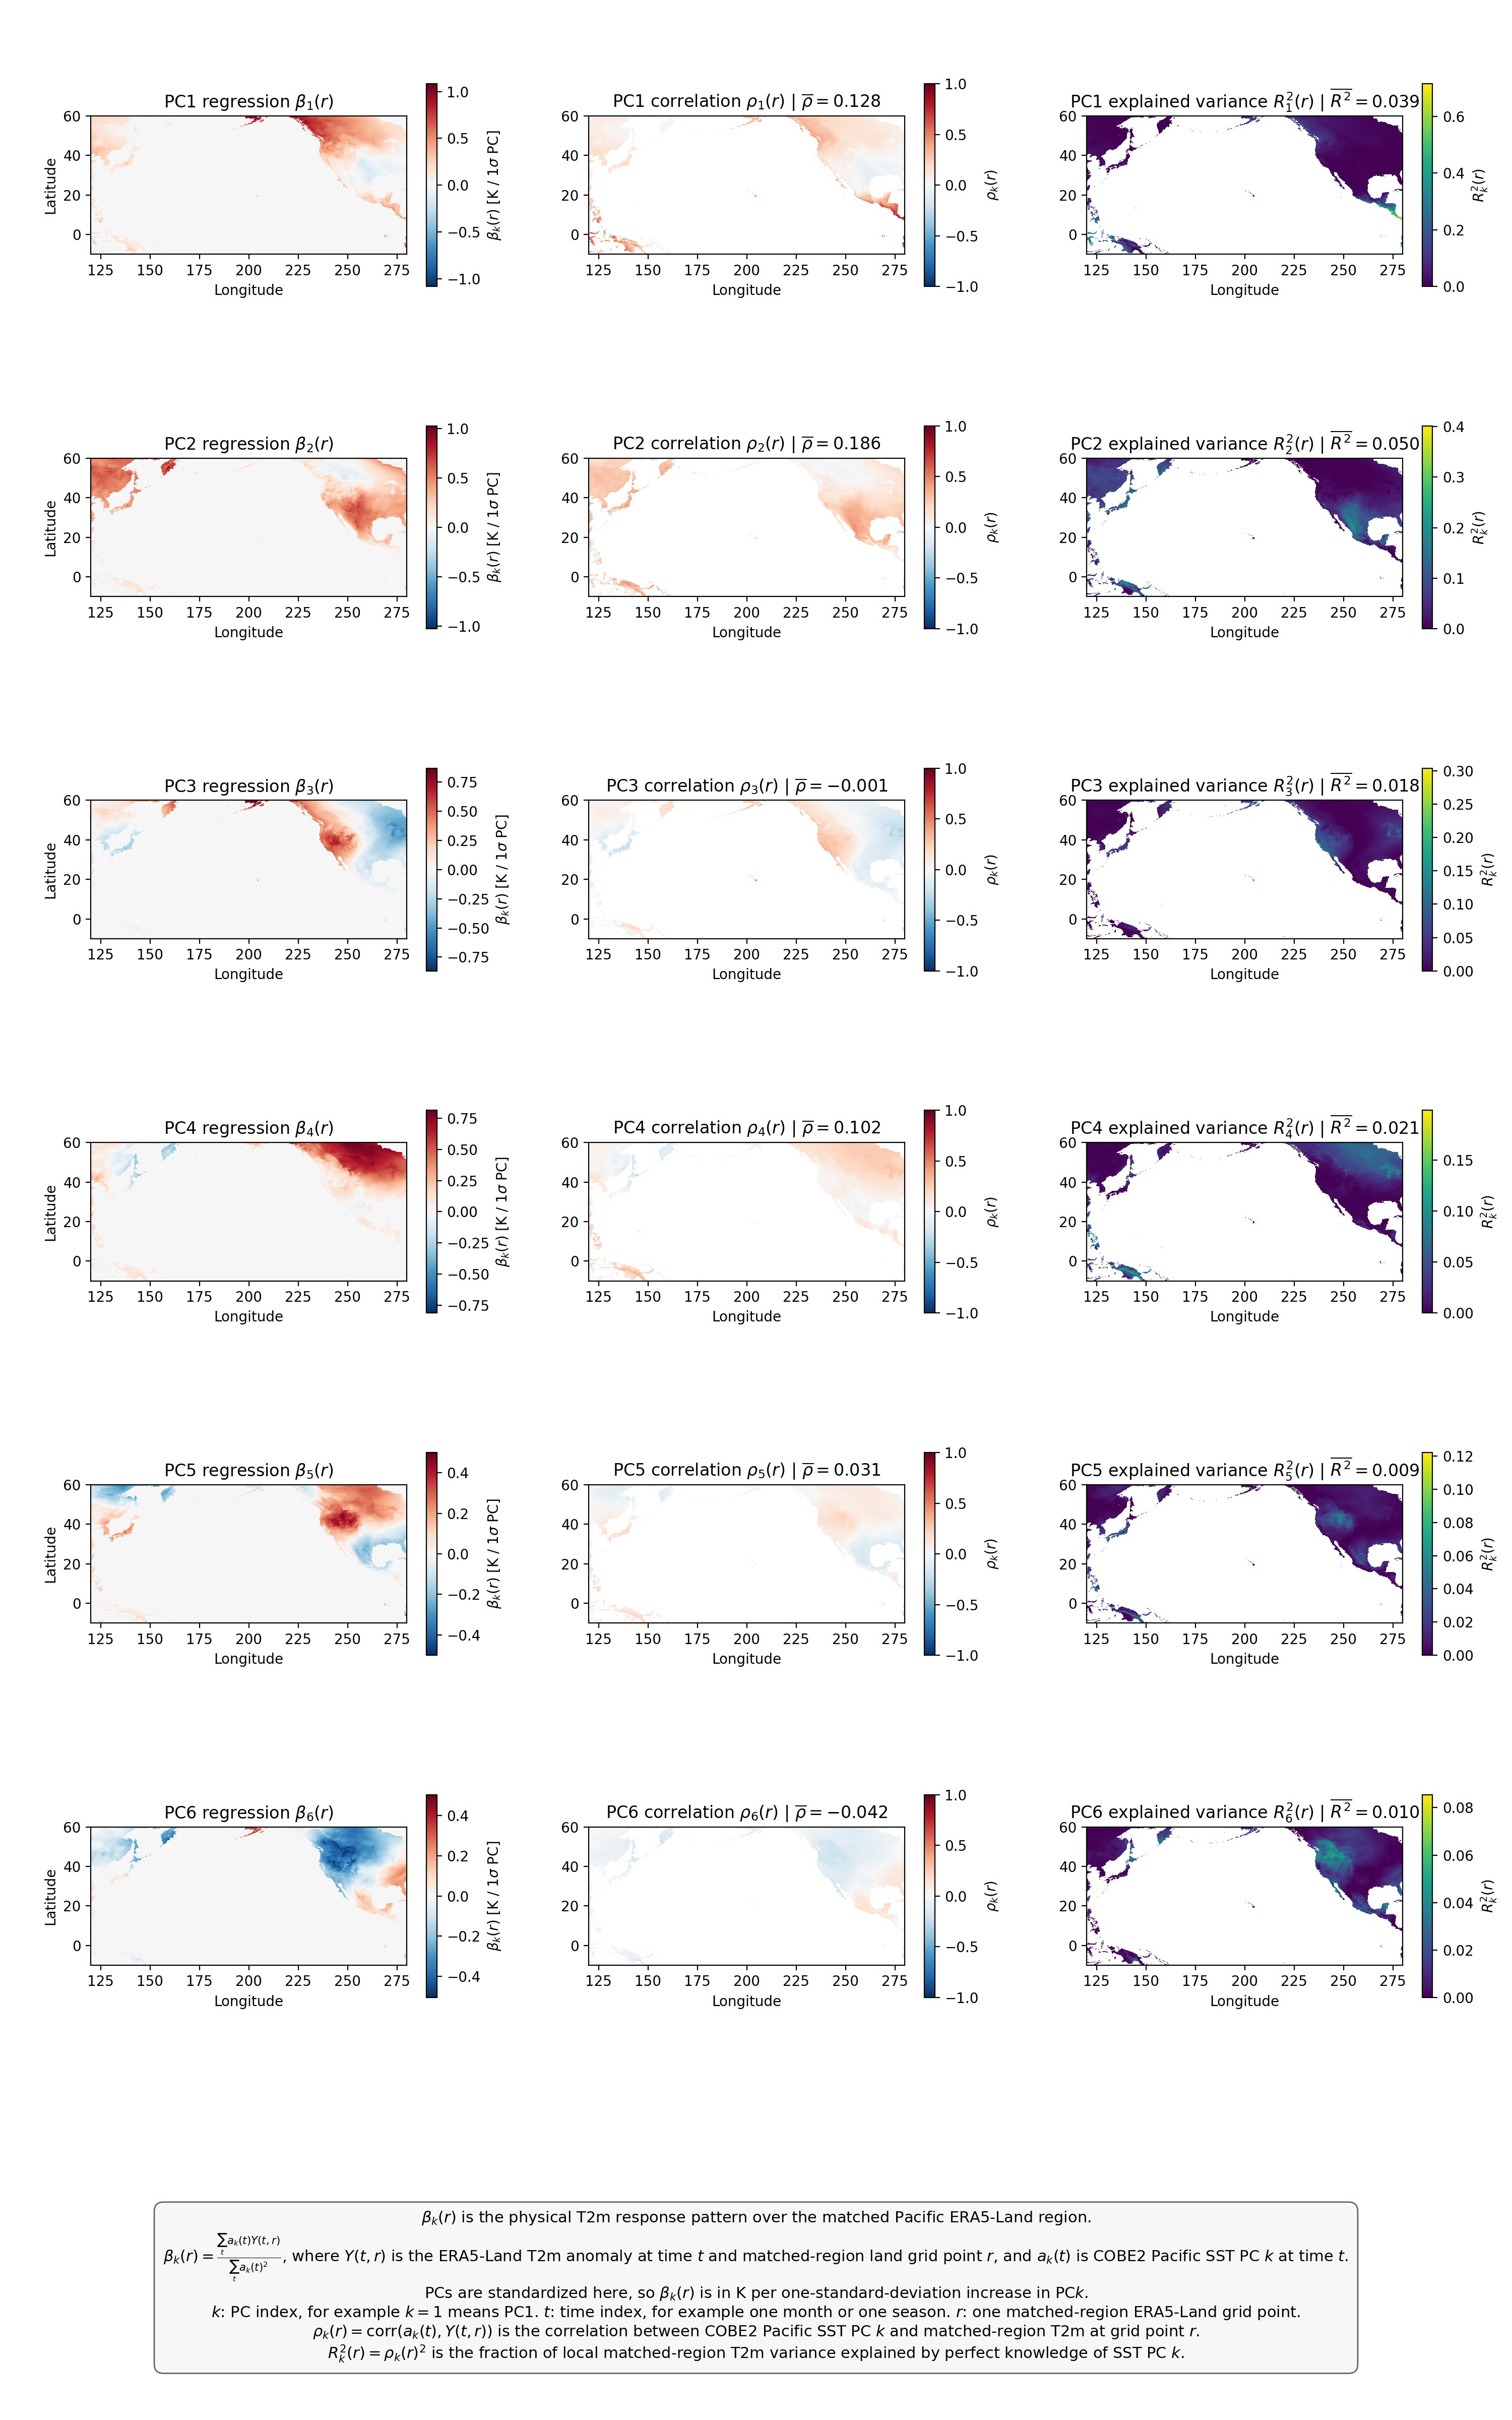
\includegraphics[width=0.49\linewidth]{../figures/cobe2_pacific_sierra_t2m_level1_maps_modes1to6.png}
\caption{Observed Pacific-region SST EOF and T2m-response diagnostics for modes 1--6. Left:
regional COBE2 EOF patterns over latitude $-10^\circ$ to $60^\circ$ and longitude $120^\circ$ to
$280^\circ$ in $0..360$ coordinates. Right: corresponding level-1 $\beta_k(r)$, $\rho_k(r)$, and
$R_k^2(r)$ maps from standardized-PC projection onto ERA5-Land monthly T2m anomalies over the same
region. Source plotting script: \texttt{scripts/run\_cobe2\_pacific\_sierra\_t2m\_level1\_diagnostic.py}.}
\label{fig:observed_level1_maps}
\end{figure}

\subsection{Six-PC Total Explained Variance}
\label{subsec:obs_total_evr}

The first six PCs are also used jointly in a multivariate regression over the same Pacific-region
overlap domain. Let
\begin{equation}
A(t,:) = \left[a_1(t), a_2(t), \dots, a_6(t)\right]
\end{equation}
denote the standardized six-PC predictor row at time $t$, and let $Y(t,r)$ denote the ERA5-Land
T2m anomaly field. The fitted coefficient matrix is
\begin{equation}
\hat{B} = (A^\top A)^{-1} A^\top Y,
\label{eq:bhat_multi}
\end{equation}
This is the normal-equation form of the same least-squares fit. In the code, the regression is
solved numerically with \texttt{np.linalg.lstsq}, which is the computational implementation of this
same least-squares problem rather than a different model. This is the all-overlap fit used for the
figure in this subsection. In other words, the plotted six-PC map is generated from a single
regression over the full overlap period, not from the month-restricted fits discussed later in
Section~\ref{subsec:obs_monthly_evr}. The month-specific notation $\widehat{B}_m$ applies only to
the monthly sensitivity figure; here the relevant object is the single full-period coefficient
matrix $\widehat{B}$.

We need this joint six-PC step because the single-PC maps in the previous subsection answer a
different question: they show how each SST mode looks when examined one at a time. The six-PC fit
asks the harder and more useful question of how much of the land T2m anomaly field can be explained
when the leading SST modes act together. In that setting, the role of $\widehat{B}$ is to assign
one coefficient map to each PC while accounting for the simultaneous presence of the other retained
PCs in the same regression.

Here, each row of $\hat{B}$ has a direct interpretation:
\begin{itemize}[leftmargin=1.5em]
  \item $\hat{B}_{1}(r)$ tells us how much the local T2m anomaly at grid point $r$ changes when PC1 increases by one standard deviation, while PCs 2--6 are held fixed in the fit.
  \item $\hat{B}_{2}(r)$ is interpreted the same way for PC2.
  \item More generally, each $\hat{B}_{k}(r)$ isolates the contribution of PC $k$ by fitting all six PCs together rather than one at a time.
\end{itemize}
Because the PCs are standardized in the six-PC workflow, each $\hat{B}_{k}(r)$ is interpreted as
kelvin per one-standard-deviation increase in PC $k$, holding the other retained PCs fixed. The
reconstructed field is
\begin{equation}
\hat{Y}(t,r) = \sum_{k=1}^{6} a_k(t)\,\hat{B}_{k}(r),
\label{eq:yhat_multi}
\end{equation}
and the local six-PC explained-variance map is
\begin{equation}
R^2(r) = 1 - \frac{\sum_t \left[Y(t,r)-\hat{Y}(t,r)\right]^2}{\sum_t Y(t,r)^2}.
\label{eq:r2_multi}
\end{equation}
This $R^2(r)$ is the fraction of local T2m variance jointly explained by the six standardized SST
PCs. In the current repo, this six-PC observed diagnostic is implemented in
\texttt{scripts/run\_cobe2\_pacific\_sierra\_t2m\_level2\_pc1to6.py}.

\begin{figure}[h]
\centering
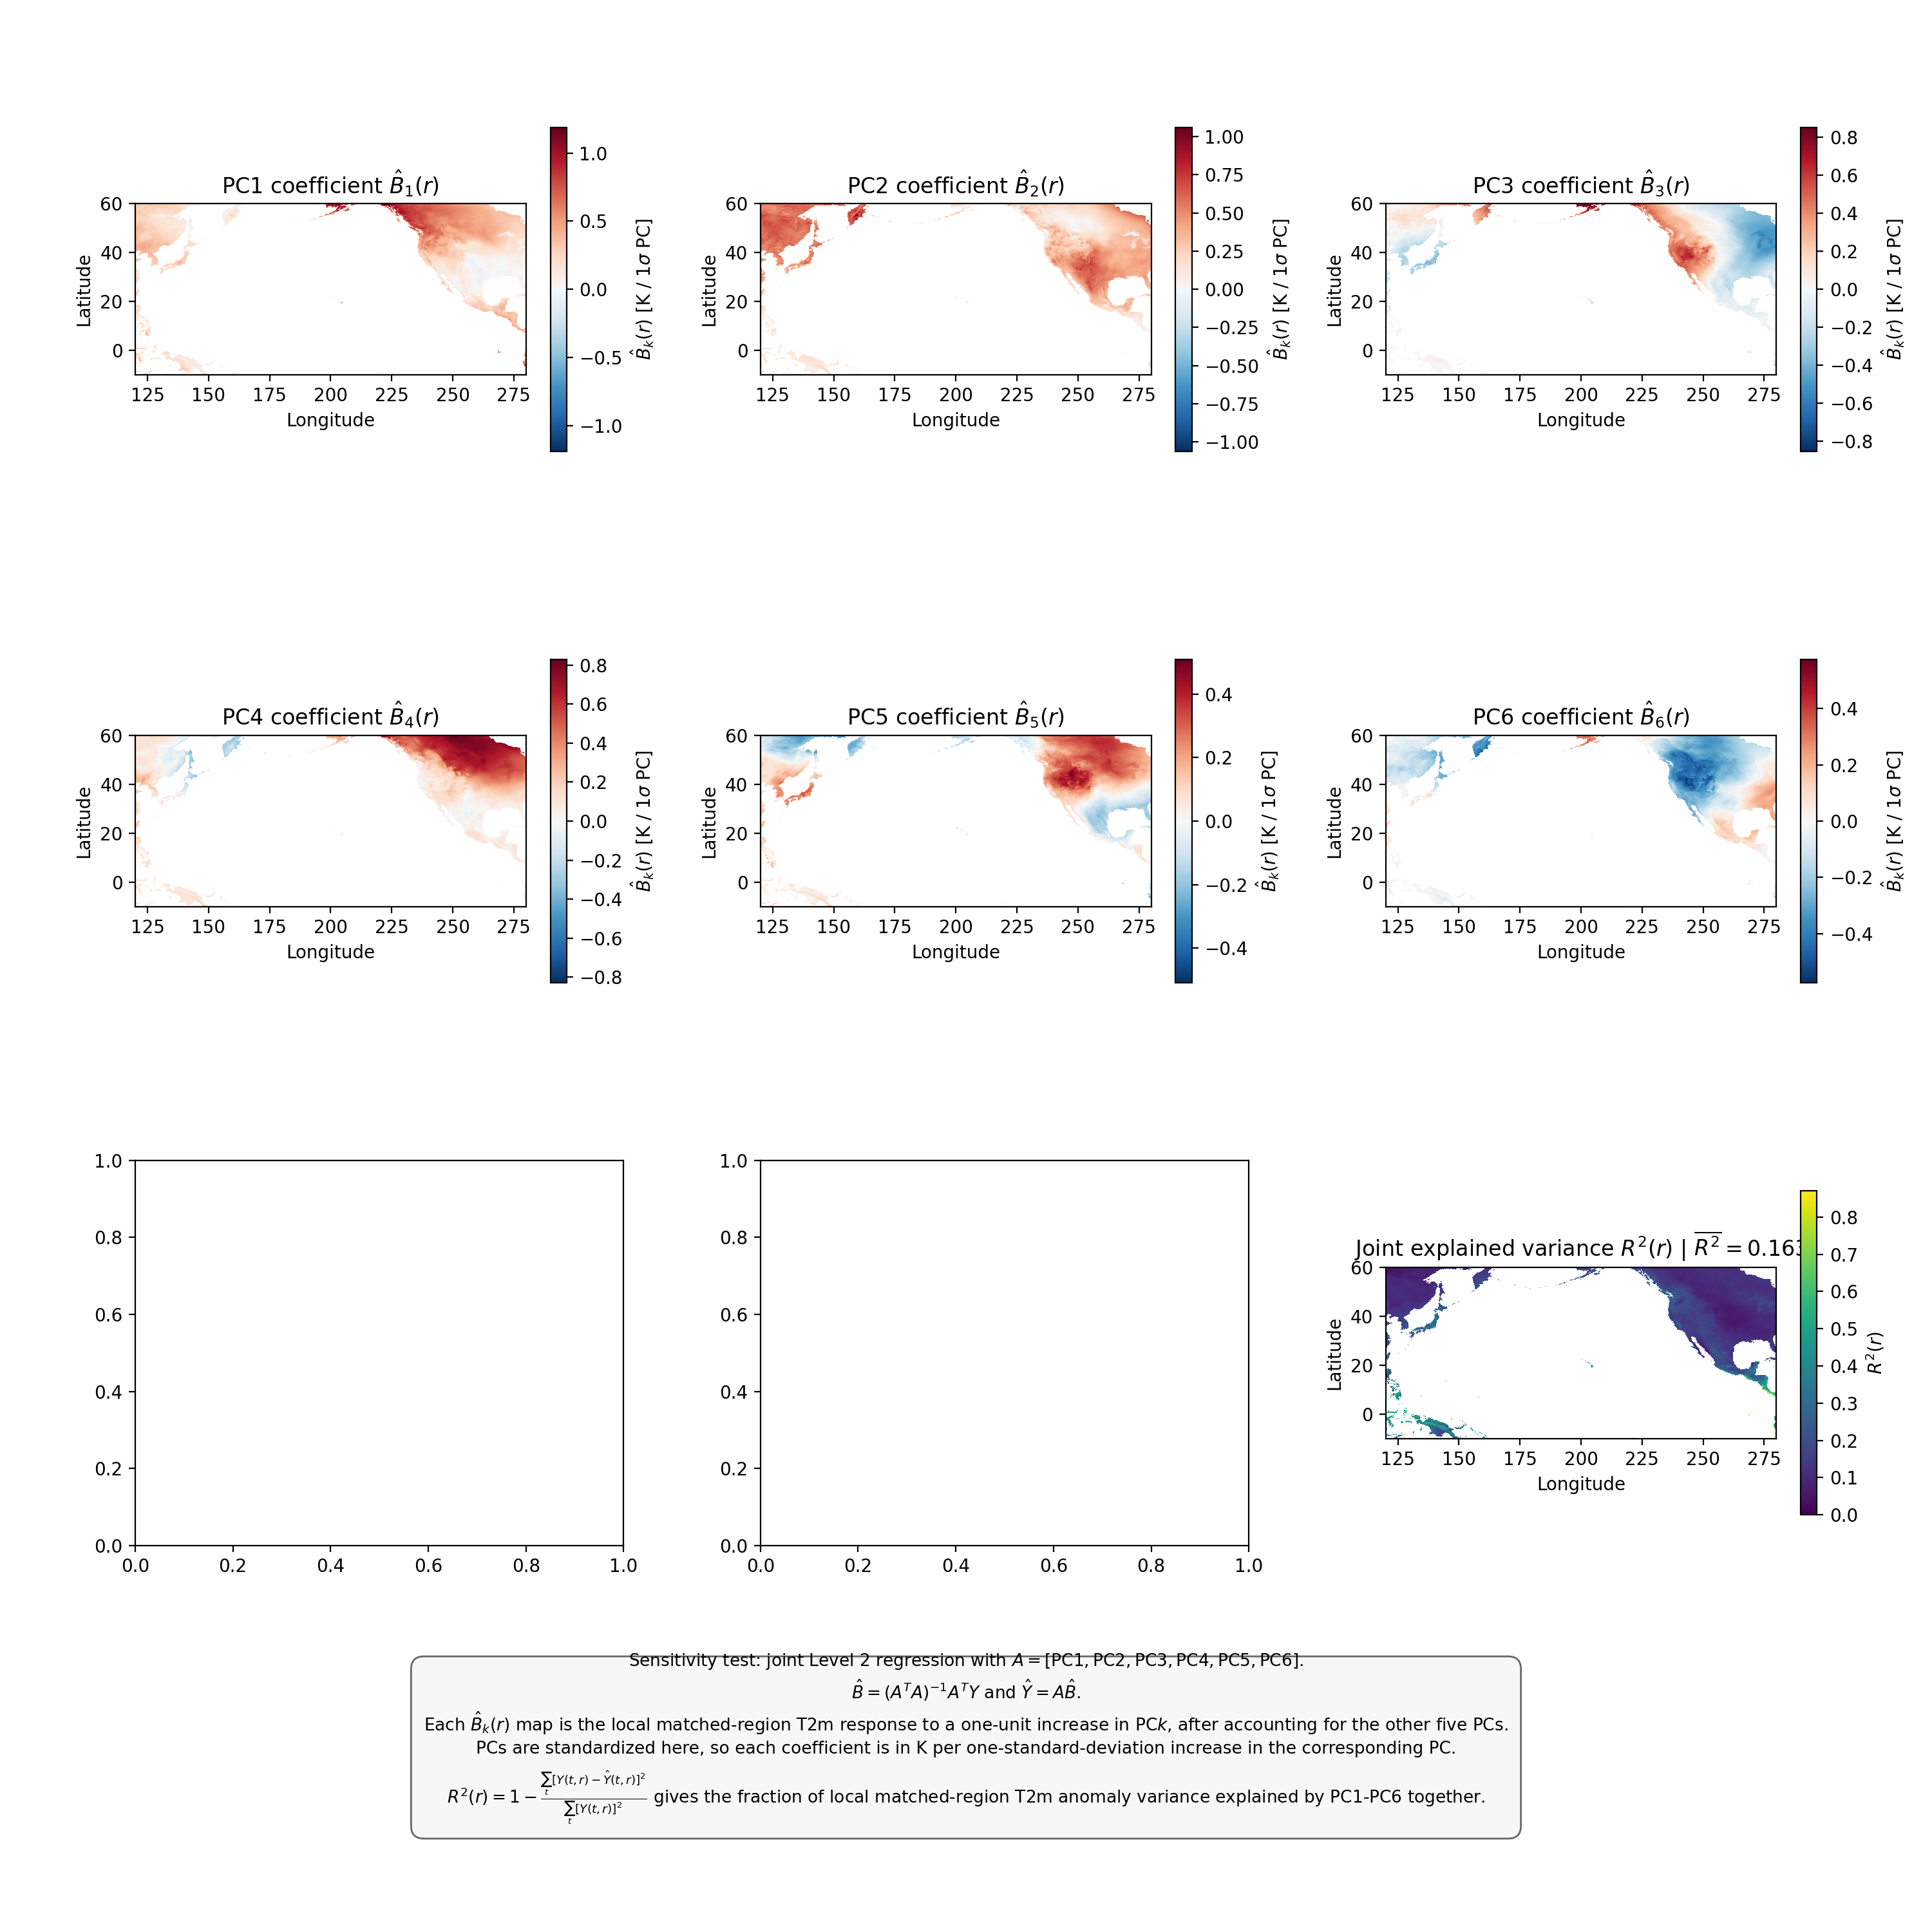
\includegraphics[width=0.82\linewidth]{../figures/cobe2_pacific_sierra_t2m_level2_pc1to6_maps.png}
\caption{Observed six-PC multivariate SST--T2m diagnostic over the Pacific-region analysis domain.
The coefficient maps correspond to the rows of $\hat{B}$ in Eq.~\eqref{eq:bhat_multi}, so each
panel shows the partial T2m response pattern for one standardized SST PC while holding the other
retained PCs fixed. The $R^2(r)$ panel summarizes the local variance jointly explained by PCs 1--6.
Source plotting script: \texttt{scripts/run\_cobe2\_pacific\_sierra\_t2m\_level2\_pc1to6.py}.}
\label{fig:observed_level2_maps}
\end{figure}

\subsection{Monthly Explained Variance}
\label{subsec:obs_monthly_evr}

We run the same six-PC regression on a restricted monthly subset and measure how much of the
Sierra-region-only monthly overland T2m anomaly variance can be explained in that subset. The
plotted quantity is the EVR, equivalently the six-PC $R^2$ map for the chosen month. The script is
located at
\texttt{scripts/run\_cobe2\_pacific\_sierra\_t2m\_level2\_pc1to6\_seasonal\_sensitivity.py}.

We use the stored standardized PC1--PC6 overlap time series from
\texttt{cobe2\_pacific\_sierra\_t2m\_level2\_pc1to6.nc}. We also use the same Pacific region:
latitude $-10^\circ$ to $60^\circ$ and longitude $120^\circ$ to $280^\circ$ in $0..360$
coordinates. The ERA5-Land target field is built over the same Pacific region, using the monthly
T2m anomaly field. However, after the reconstructed T2m anomaly field is obtained, the EVR is
calculated only over the Sierra box, between $35^\circ$ and $42^\circ$N and between $236^\circ$ and
$243^\circ$E.

Each panel is fit only on its own month. In this monthly figure, each panel restricts $t$ to one
calendar month only. For January,
\begin{equation}
t_i \in
\left\{
\text{Jan 1949},
\text{Jan 1950},
\ldots,
\text{Jan 2022}
\right\}.
\end{equation}
For February,
\begin{equation}
t_i \in
\left\{
\text{Feb 1949},
\text{Feb 1950},
\ldots,
\text{Feb 2022}
\right\}.
\end{equation}
Therefore, the January $R^2$ calculation never uses February, March, April, or any other month.

For a selected calendar month $m$, let $A_m$ denote the standardized PC1--PC6 predictor matrix
restricted to that month, and let $Y_m$ denote the corresponding ERA5-Land monthly T2m anomaly
matrix over the Sierra evaluation cells. The same six-PC coefficient formula from the total
explained variance calculation is used, but now on the month-restricted matrices:
\begin{equation}
\widehat{B}_m
=
\left(A_m^\top A_m\right)^{-1} A_m^\top Y_m .
\end{equation}
The reconstructed monthly T2m anomaly field is
\begin{equation}
\widehat{Y}_m
=
A_m \widehat{B}_m .
\end{equation}
The plotted EVR, or local $R^2$, is then calculated at each Sierra grid cell $r$ as
\begin{equation}
R_m^2(r)
=
1
-
\frac{
\sum_{t \in m}
\left[
Y_m(t,r)-\widehat{Y}_m(t,r)
\right]^2
}{
\sum_{t \in m}
Y_m(t,r)^2
}.
\end{equation}

For a single Sierra grid cell $r$, the January panel is generated as follows. First, all January
samples are collected:
\begin{equation}
t_1 = \text{Jan 1949}, \quad
t_2 = \text{Jan 1950}, \quad
\ldots, \quad
t_{74} = \text{Jan 2022}.
\end{equation}
Then the January predictor matrix is built:
\begin{equation}
A_{\mathrm{Jan}}
=
\begin{bmatrix}
PC_1(t_1) & \cdots & PC_6(t_1) \\
PC_1(t_2) & \cdots & PC_6(t_2) \\
\vdots & \ddots & \vdots \\
PC_1(t_{74}) & \cdots & PC_6(t_{74})
\end{bmatrix}.
\end{equation}
The January target vector at grid cell $r$ is
\begin{equation}
y_{\mathrm{Jan}}(r)
=
\begin{bmatrix}
Y_{\mathrm{Jan}}(t_1,r) \\
Y_{\mathrm{Jan}}(t_2,r) \\
\vdots \\
Y_{\mathrm{Jan}}(t_{74},r)
\end{bmatrix}.
\end{equation}
For all Sierra grid cells together, this gives the January target matrix $Y_{\mathrm{Jan}}$. The
January coefficient matrix is then calculated by
\begin{equation}
\widehat{B}_{\mathrm{Jan}}
=
\left(A_{\mathrm{Jan}}^\top A_{\mathrm{Jan}}\right)^{-1}
A_{\mathrm{Jan}}^\top
Y_{\mathrm{Jan}} .
\end{equation}
The January T2m anomaly field is reconstructed as
\begin{equation}
\widehat{Y}_{\mathrm{Jan}}
=
A_{\mathrm{Jan}}
\widehat{B}_{\mathrm{Jan}} .
\end{equation}
At grid cell $r$, the January EVR is
\begin{equation}
R^2_{\mathrm{Jan}}(r)
=
1
-
\frac{
\sum_{i=1}^{74}
\left[
Y_{\mathrm{Jan}}(t_i,r)
-
\widehat{Y}_{\mathrm{Jan}}(t_i,r)
\right]^2
}{
\sum_{i=1}^{74}
Y_{\mathrm{Jan}}(t_i,r)^2
}.
\end{equation}

This single value becomes the color at grid cell $r$ in the January panel. Repeating this for every
Sierra grid cell gives the January map. Repeating the same process for February, March, April, and
the remaining months gives the twelve monthly panels.

\begin{figure}[h]
\centering
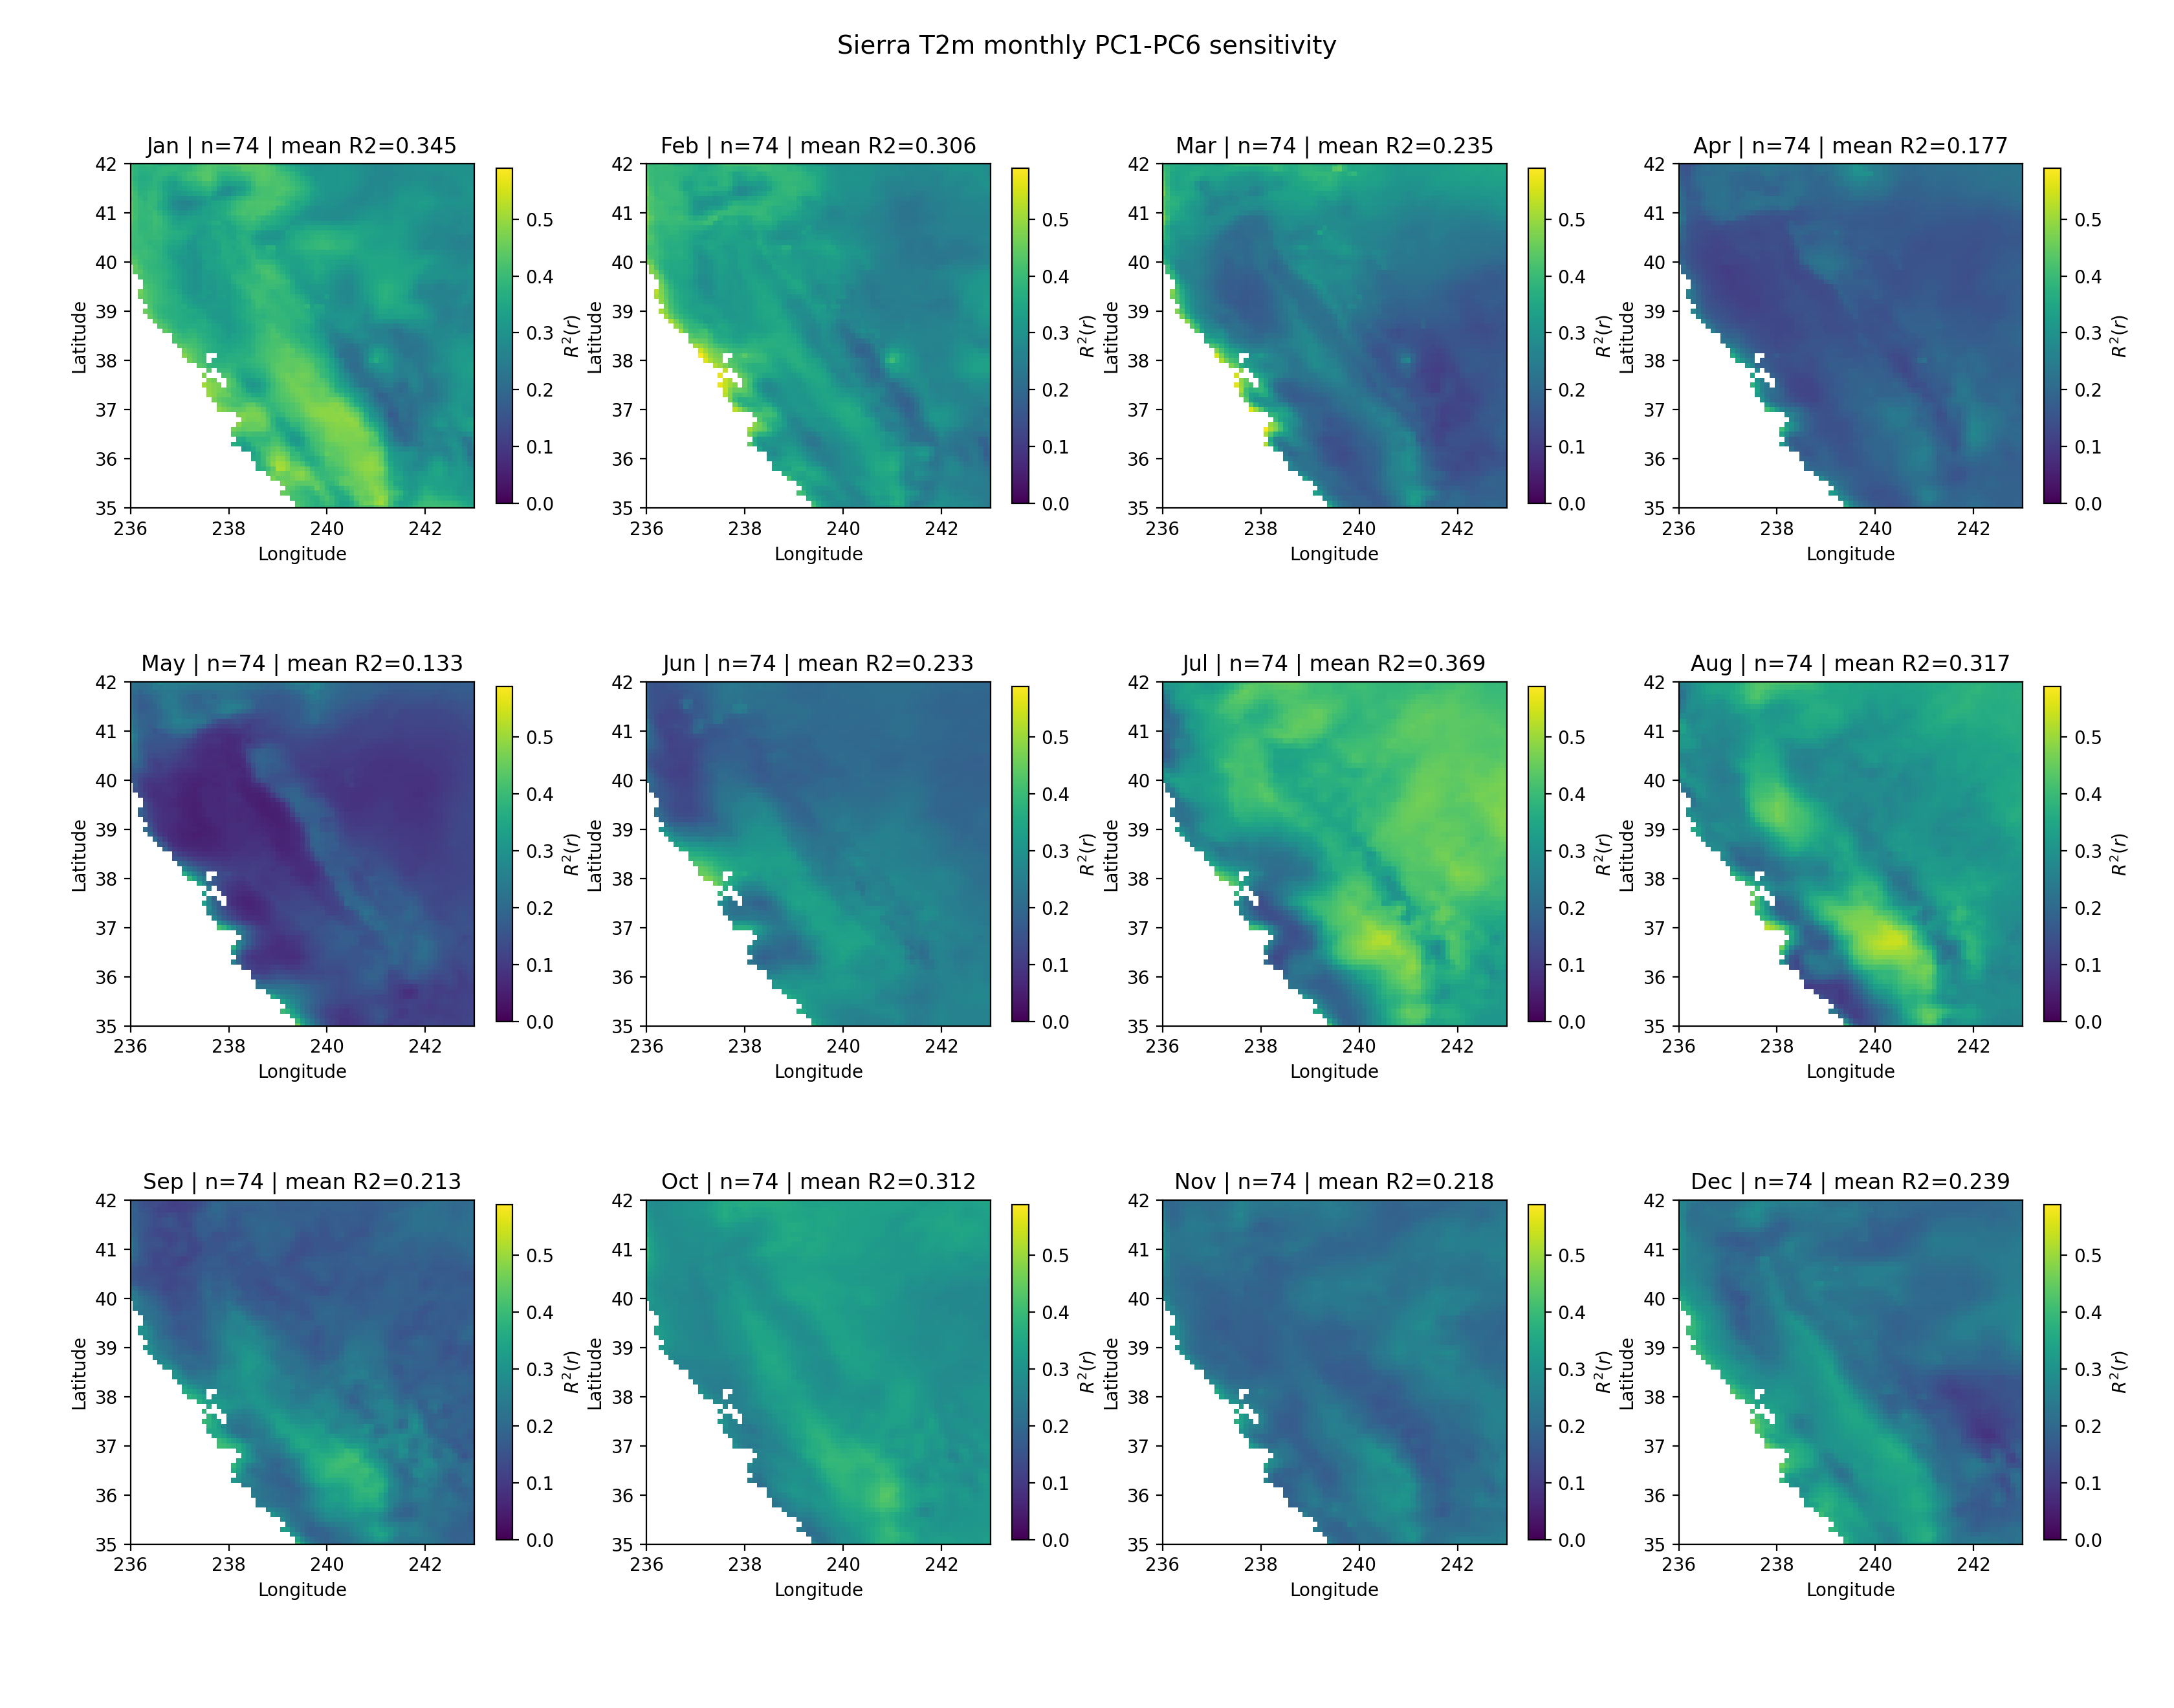
\includegraphics[width=0.88\linewidth]{../figures/cobe2_pacific_sierra_t2m_level2_pc1to6_monthly_r2_maps.png}
\caption{Monthly six-PC $R^2(r)$ maps over the Sierra evaluation region. Each panel is fit using
only the overlap samples from that calendar month. The predictors are standardized COBE2 SST
PC1--PC6 from the expanded Pacific-domain run, and the target is ERA5-Land monthly T2m anomaly
evaluated over the Sierra box. Source plotting script:
\texttt{scripts/run\_cobe2\_pacific\_sierra\_t2m\_level2\_pc1to6\_seasonal\_sensitivity.py}.}
\label{fig:monthly_r2_maps}
\end{figure}

The current monthly result shows that the SST-PC linkage to Sierra T2m is stronger in winter and
summer. December, January, February, and March are relatively strong, and June through August also
show high values, with July and August among the largest monthly mean $R^2$ values in the current
summary.

\section{SST-PC Response in WUSD-03}
\label{sec:wusd}

The WUSD-03 SST field is not defined over the full Pacific predictor domain used for the COBE2 EOF
analysis. In this workflow, the COBE2 modes are built over the broad Pacific box
($120^\circ$--$280^\circ$E, $10^\circ$S--$60^\circ$N), while the WUSD-03 SST coverage only appears
over the subset of that box reached by the model's d01 ocean points after regridding. As a result,
the WUSD-03 projection cannot use the full COBE2 EOF support. It instead uses only the shared SST
region where COBE2 has valid ocean data and the remapped WUSD-03 SST is finite.

\begin{figure}[h]
\centering
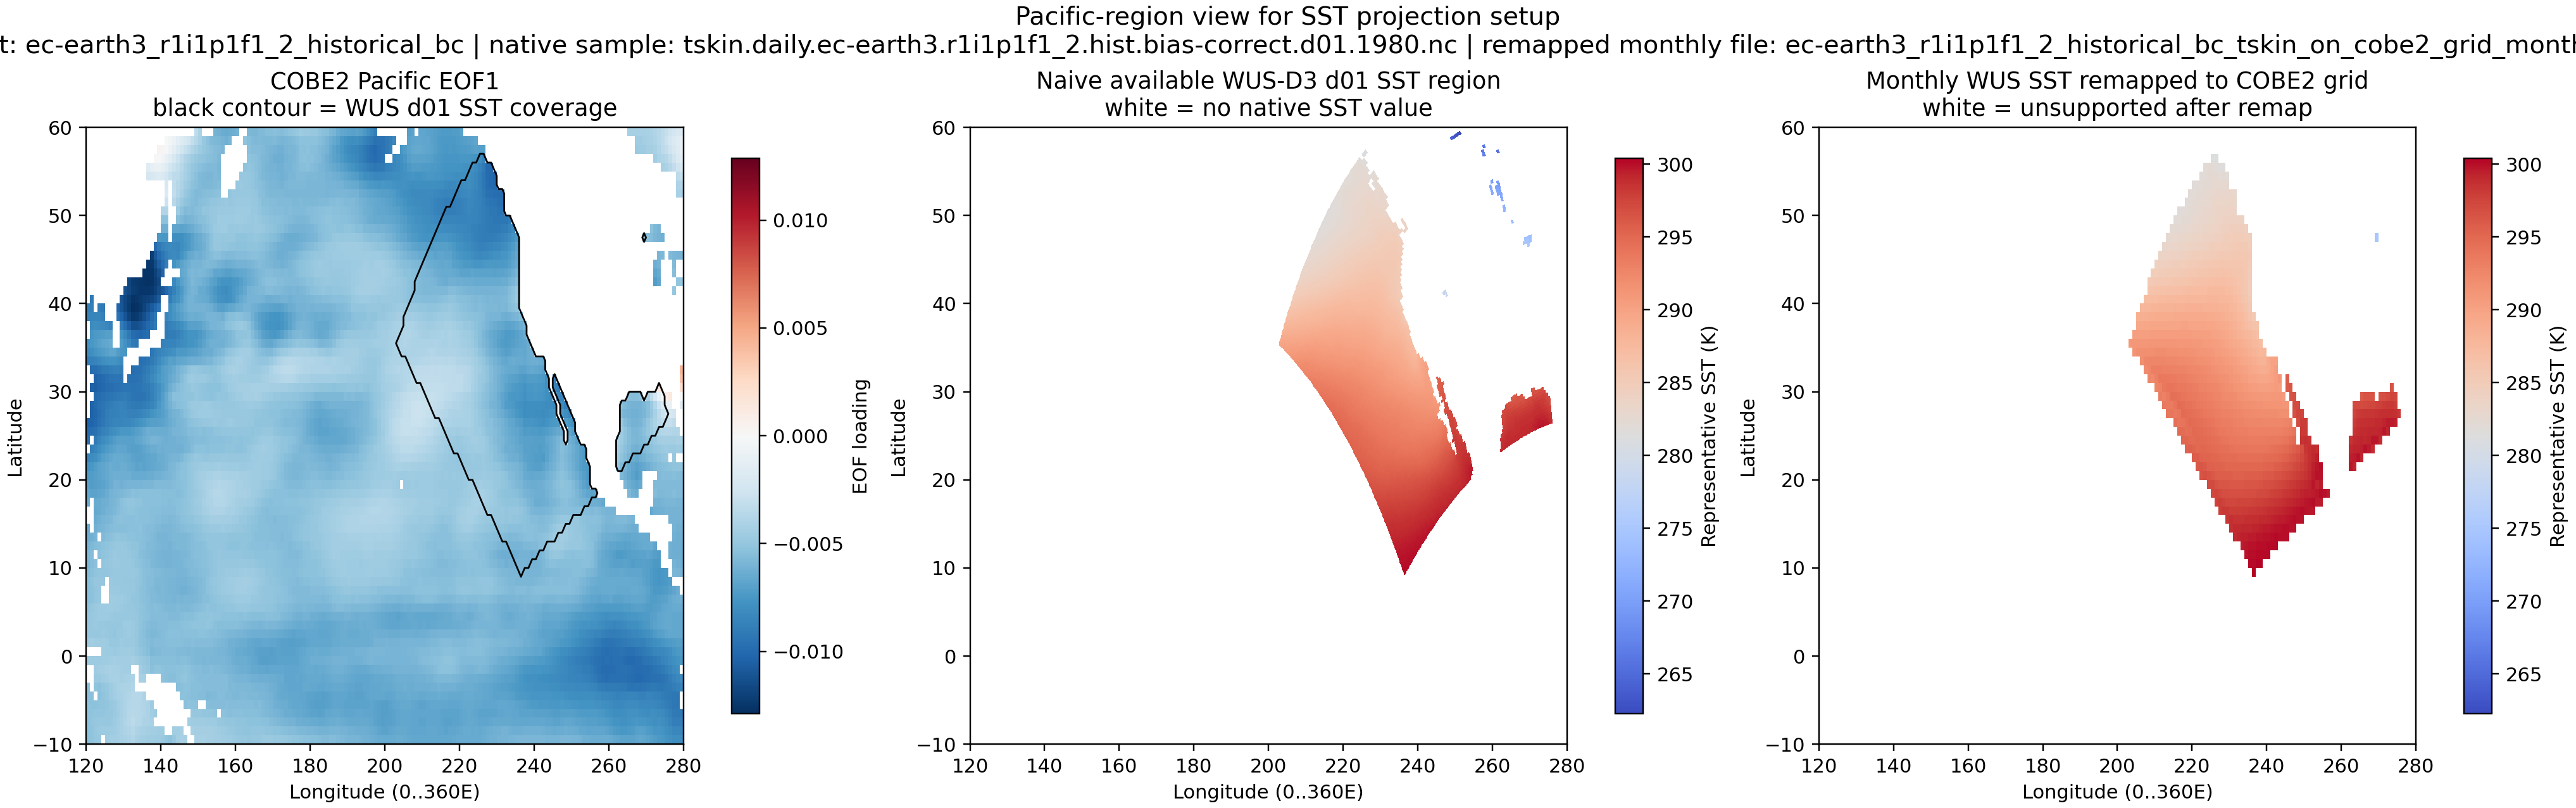
\includegraphics[width=0.95\linewidth]{../figures/cobe2_eof1_and_wusd3_d01_pacific_coverage.png}
\caption{Pacific-domain coverage mismatch for the WUSD-03 SST projection setup. The left panel
shows COBE2 EOF1 over the full Pacific predictor domain, with the black contour marking the part
of that domain where WUSD-03 d01 contributes SST after regridding. The right panel shows the same
WUSD-03 SST coverage directly: only a limited eastern and northeastern Pacific subset is available,
while the white area is missing or outside the WUSD-03 SST footprint. This is why the WUSD-03
projection uses a shared mask rather than the full COBE2 Pacific domain. Source plotting script:
\texttt{scripts/plot\_cobe2\_eof1\_and\_wusd3\_d01\_pacific\_coverage.py}.}
\label{fig:wusd_pacific_coverage}
\end{figure}

\subsection{Shared-Region Observational Reference}
\label{subsec:wusd_sharedregion_obs}

This shared-region observational reference answers the following question:
\begin{quote}
If the observational SST information were restricted to the same ocean region available in
WUSD-03, what SST modes would COBE2 produce, and how much Sierra T2m variance would those regional
SST modes explain?
\end{quote}

Figure~\ref{fig:wusd_pacific_coverage} is produced by
\path{scripts/plot_cobe2_eof1_and_wusd3_d01_pacific_coverage.py}, which visualizes the
Pacific-domain mismatch between the full COBE2 EOF box and the remapped WUSD-03 d01 SST footprint.
The shared-region processing itself is then carried out by
\path{scripts/run_cobe2_sharedregion_wusd3_sierra_t2m_diagnostics.py}, which restricts
COBE2 SST to the valid WUSD-03 coverage, recomputes the shared-region COBE2 EOF basis, projects
WUSD-03 SST onto that basis, and builds the corresponding Sierra T2m diagnostics.

To construct the shared-region observational reference, we first define a shared SST region $M$,
corresponding to the COBE2 grid cells that fall inside the valid WUSD-03 d01 SST coverage. We then
extract COBE2 monthly SST only over this shared region:
\begin{equation}
\sst_{\mathrm{COBE2},M}(x,t),
\qquad x \in M.
\end{equation}

The SST anomalies are computed using the same monthly-climatology convention as in the full-Pacific
COBE2 EOF workflow:
\begin{equation}
\sst_{\mathrm{COBE2},M}^{\prime}(x,t)
=
\sst_{\mathrm{COBE2},M}(x,t)
- \overline{\sst}_{\mathrm{COBE2},M,m(t)}(x),
\qquad x \in M,
\label{eq:cobe2_sharedregion_anomaly}
\end{equation}
where $\overline{\sst}_{\mathrm{COBE2},M,m}(x)$ is the month-of-year climatological mean at grid
cell $x$ for calendar month $m$.

After anomaly construction, the shared-region COBE2 anomaly field is reshaped into a time--space
matrix:
\begin{equation}
X_{\mathrm{COBE2},M}(t,x)
=
\sst_{\mathrm{COBE2},M}^{\prime}(x,t),
\qquad x \in M.
\end{equation}

We then repeat the same EOF/PCA treatment used in the previous COBE2 EOF workflow, but now using
only the shared WUSD-03 SST coverage region. In particular, the shared-region anomaly matrix is
area-weighted using the same latitude-weighting convention as before, and no new EOF information
from WUSD-03 is used. The EOF/PCA solve is performed entirely on COBE2 SST restricted to $M$. This
gives a new set of regional COBE2 SST modes:
\begin{equation}
\sst_{\mathrm{COBE2},M}^{\prime}(x,t)
\approx
\sum_{k=1}^{6}
P^{\mathrm{COBE2},M}_{k}(t)\,E^{\mathrm{COBE2},M}_{k}(x),
\qquad x \in M.
\label{eq:cobe2_sharedregion_eof_expansion}
\end{equation}

Here, $E^{\mathrm{COBE2},M}_{k}(x)$ is the $k$-th COBE2 EOF pattern computed only over the
shared WUSD-03 SST region, and $P^{\mathrm{COBE2},M}_{k}(t)$ is the corresponding COBE2
shared-region PC time series. These are not the same as the full-Pacific COBE2 EOFs and PCs. They
are a new observational PCA basis obtained from COBE2 SST after restricting the SST field to the
WUSD-03 d01 ocean coverage.

Before using the shared-region PCs in the T2m response analysis, each PC is standardized over the
overlap period, following the same convention used in the previous observational Level-1 and
Level-2 diagnostics:
\begin{equation}
a^{\mathrm{COBE2},M}_{k}(t)
=
\frac{
P^{\mathrm{COBE2},M}_{k}(t) - \overline{P^{\mathrm{COBE2},M}_{k}}
}{
\mathrm{std}\!\left(P^{\mathrm{COBE2},M}_{k}\right)
}.
\label{eq:cobe2_sharedregion_pc_standardization}
\end{equation}
Thus, the response coefficients are interpreted as kelvin per one-standard-deviation increase in
the corresponding shared-region COBE2 PC.

Using these standardized shared-region COBE2 PCs, we repeat the same Level-2 monthly explained
variance calculation described in Section~\ref{subsec:obs_monthly_evr}. For each calendar month
$m$, we build the month-restricted predictor matrix
\begin{equation}
A_{\mathrm{COBE2},M,m}(t,:)
=
\left[
a^{\mathrm{COBE2},M}_{1}(t),
a^{\mathrm{COBE2},M}_{2}(t),
\dots,
a^{\mathrm{COBE2},M}_{6}(t)
\right],
\qquad t \in m,
\end{equation}
and the corresponding ERA5-Land Sierra T2m anomaly target matrix
\begin{equation}
Y_{\mathrm{ERA5},m}(t,r),
\qquad t \in m.
\end{equation}

For each calendar month, the six-PC coefficient matrix is computed by the same ordinary least
squares formula:
\begin{equation}
\widehat{B}_{\mathrm{COBE2},M,m}
=
\left(
A_{\mathrm{COBE2},M,m}^{\top}
A_{\mathrm{COBE2},M,m}
\right)^{-1}
A_{\mathrm{COBE2},M,m}^{\top}
Y_{\mathrm{ERA5},m}.
\label{eq:cobe2_sharedregion_monthly_bhat}
\end{equation}
As in the earlier sections, the implementation can be written analytically with the normal equation
while the numerical solve is carried out with \texttt{np.linalg.lstsq} in
\path{scripts/run_cobe2_sharedregion_wusd3_sierra_t2m_diagnostics.py}.

The reconstructed ERA5-Land Sierra T2m anomaly field is
\begin{equation}
\widehat{Y}_{\mathrm{ERA5},M,m}
=
A_{\mathrm{COBE2},M,m}
\widehat{B}_{\mathrm{COBE2},M,m}.
\label{eq:cobe2_sharedregion_monthly_yhat}
\end{equation}

The local monthly explained variance is then
\begin{equation}
R^{2}_{\mathrm{COBE2},M,m}(r)
=
1
-
\frac{
\sum_{t \in m}
\left[
Y_{\mathrm{ERA5},m}(t,r) - \widehat{Y}_{\mathrm{ERA5},M,m}(t,r)
\right]^2
}{
\sum_{t \in m}
Y_{\mathrm{ERA5},m}(t,r)^2
}.
\label{eq:cobe2_sharedregion_monthly_r2}
\end{equation}

The resulting monthly $R^2$ maps show how much Sierra T2m variance is explained by the first six
COBE2 SST PCs when the COBE2 SST information is restricted to the same region available in WUSD-03.
This figure therefore serves as the masked/shared-region observational reference for the WUSD-03
comparison.

\begin{figure}[h]
\centering
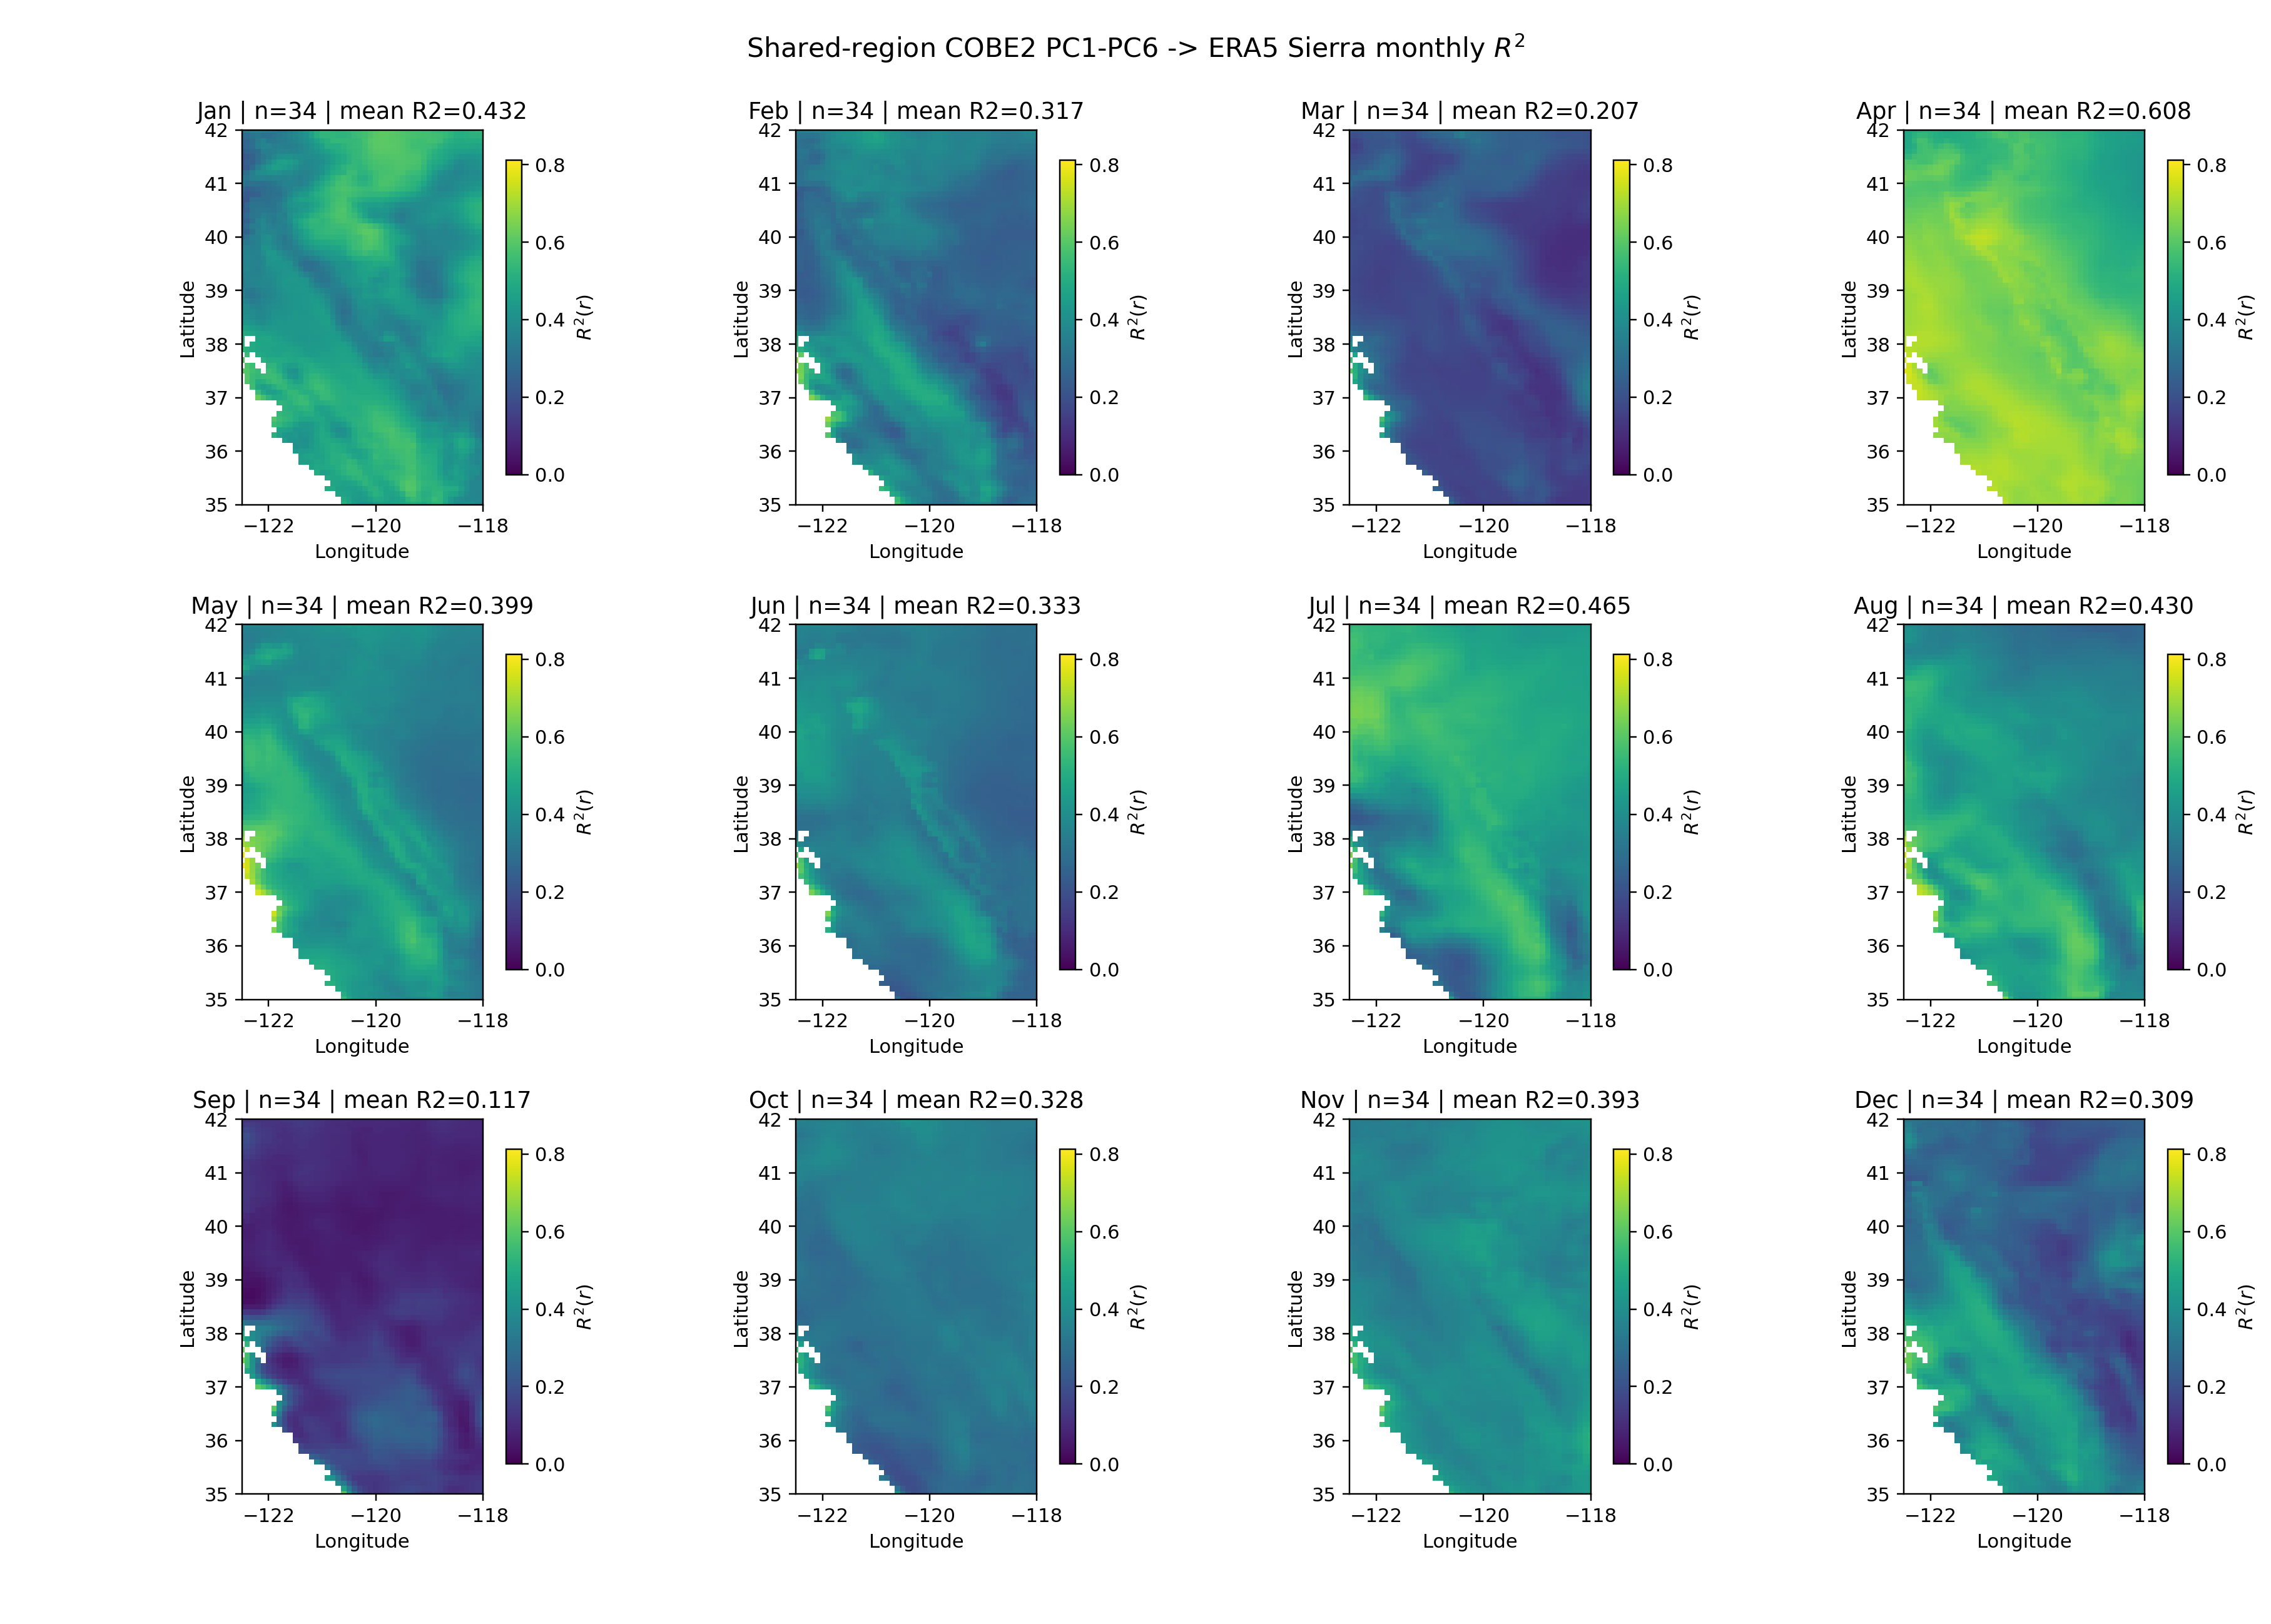
\includegraphics[width=0.88\linewidth]{../figures/cobe2_sharedregion_sierra_t2m_level2_pc1to6_monthly_r2_maps.png}
\caption{Monthly six-PC $R^2(r)$ maps over the Sierra evaluation region using COBE2 SST restricted
to the WUSD-03 d01 SST coverage. The SST EOFs and PCs are recomputed from COBE2 SST anomalies over
the shared region $M$, rather than using the full-Pacific COBE2 EOFs. Each panel is fit using only
samples from that calendar month. The predictors are the standardized shared-region COBE2 PCs
1--6, and the target is ERA5-Land monthly T2m anomaly over the Sierra box. Source generating
script: \texttt{scripts/run\_cobe2\_sharedregion\_wusd3\_sierra\_t2m\_diagnostics.py}.}
\label{fig:cobe2_sharedregion_monthly_r2_maps}
\end{figure}

\subsection{WUSD-03 SST Projection onto Shared-Region COBE2 EOFs}
\label{subsec:wusd3_projection_sharedregion_cobe2_eofs}

After constructing the shared-region COBE2 EOF basis, we use it as the observational SST
coordinate system for WUSD-03. The goal is not to compute new EOFs from WUSD-03 SST. Instead, we
ask whether WUSD-03 SST variability, when expressed in the shared-region COBE2 EOF basis, produces
a similar overland T2m response.

We begin with WUSD-03 SST over the same shared region $M$. The WUSD-03 SST anomaly field is
written as
\begin{equation}
\sst_{\mathrm{WUS},M}^{\prime}(x,t),
\qquad x \in M,
\end{equation}
where the monthly anomaly is computed using the same month-of-year anomaly convention:
\begin{equation}
\sst_{\mathrm{WUS},M}^{\prime}(x,t)
=
\sst_{\mathrm{WUS},M}(x,t)
- \overline{\sst}_{\mathrm{WUS},M,m(t)}(x).
\label{eq:wus_sharedregion_anomaly}
\end{equation}

The anomaly construction, the remapping to the COBE2 grid, the shared-region EOF solve, and the
subsequent regression diagnostics are all handled in
\path{scripts/run_cobe2_sharedregion_wusd3_sierra_t2m_diagnostics.py}. Within that
workflow, WUSD-03 monthly SST is projected onto the shared-region COBE2 EOFs computed in the
previous subsection. For each mode $k$, the projected WUSD-03 score is
\begin{equation}
z^{\mathrm{WUS},M}_{k}(t)
=
\sum_{x \in M}
\sst_{\mathrm{WUS},M}^{\prime}(x,t)\,E^{\mathrm{COBE2},M}_{k}(x).
\label{eq:wus_projected_sharedregion_pc}
\end{equation}

Equivalently, in matrix form,
\begin{equation}
Z_{\mathrm{WUS},M}
=
X_{\mathrm{WUS},M}
E_{\mathrm{COBE2},M},
\label{eq:wus_projected_sharedregion_matrix}
\end{equation}
where $X_{\mathrm{WUS},M}$ is the WUSD-03 SST anomaly matrix over the shared region and
$E_{\mathrm{COBE2},M}$ contains the first six shared-region COBE2 EOF patterns.

The resulting time series $z^{\mathrm{WUS},M}_{k}(t)$ are the WUSD-03 SST projected scores in the
shared-region COBE2 EOF coordinate system. They are the WUSD-03 counterpart to the shared-region
COBE2 PCs, but they are not EOFs computed from WUSD-03. They measure how strongly the WUSD-03 SST
anomaly field projects onto each observed shared-region COBE2 SST mode.

Following the same convention used for the observational PC predictors, each projected WUSD-03
score is standardized before the T2m response analysis:
\begin{equation}
a^{\mathrm{WUS},M}_{k}(t)
=
\frac{
z^{\mathrm{WUS},M}_{k}(t) - \overline{z^{\mathrm{WUS},M}_{k}}
}{
\mathrm{std}\!\left(z^{\mathrm{WUS},M}_{k}\right)
}.
\label{eq:wus_projected_score_standardization}
\end{equation}
Thus, the WUSD-03 response coefficients are interpreted as kelvin per one-standard-deviation
increase in the projected WUSD-03 SST score.

We then repeat the same Level-2 monthly explained variance calculation used for the observational
reference. For each calendar month $m$, the WUSD-03 predictor matrix is
\begin{equation}
A_{\mathrm{WUS},M,m}(t,:)
=
\left[
a^{\mathrm{WUS},M}_{1}(t),
a^{\mathrm{WUS},M}_{2}(t),
\dots,
a^{\mathrm{WUS},M}_{6}(t)
\right],
\qquad t \in m,
\end{equation}
and the target matrix is the WUSD-03 overland T2m anomaly field over the Sierra evaluation region:
\begin{equation}
Y_{\mathrm{WUS},m}(t,r),
\qquad t \in m.
\end{equation}

The month-specific six-PC coefficient matrix is
\begin{equation}
\widehat{B}_{\mathrm{WUS},M,m}
=
\left(
A_{\mathrm{WUS},M,m}^{\top}
A_{\mathrm{WUS},M,m}
\right)^{-1}
A_{\mathrm{WUS},M,m}^{\top}
Y_{\mathrm{WUS},m}.
\label{eq:wus_sharedregion_monthly_bhat}
\end{equation}

The reconstructed WUSD-03 Sierra T2m anomaly field is
\begin{equation}
\widehat{Y}_{\mathrm{WUS},M,m}
=
A_{\mathrm{WUS},M,m}
\widehat{B}_{\mathrm{WUS},M,m}.
\label{eq:wus_sharedregion_monthly_yhat}
\end{equation}

The local monthly explained variance is
\begin{equation}
R^{2}_{\mathrm{WUS},M,m}(r)
=
1
-
\frac{
\sum_{t \in m}
\left[
Y_{\mathrm{WUS},m}(t,r) - \widehat{Y}_{\mathrm{WUS},M,m}(t,r)
\right]^2
}{
\sum_{t \in m}
Y_{\mathrm{WUS},m}(t,r)^2
}.
\label{eq:wus_sharedregion_monthly_r2}
\end{equation}

The resulting monthly $R^2$ maps show how much WUSD-03 Sierra T2m variance is explained by the
first six WUSD-03 SST projected scores in the shared-region COBE2 EOF basis. This is the direct
model-side counterpart to the shared-region COBE2 observational reference in
Figure~\ref{fig:cobe2_sharedregion_monthly_r2_maps}.

\begin{figure}[h]
\centering
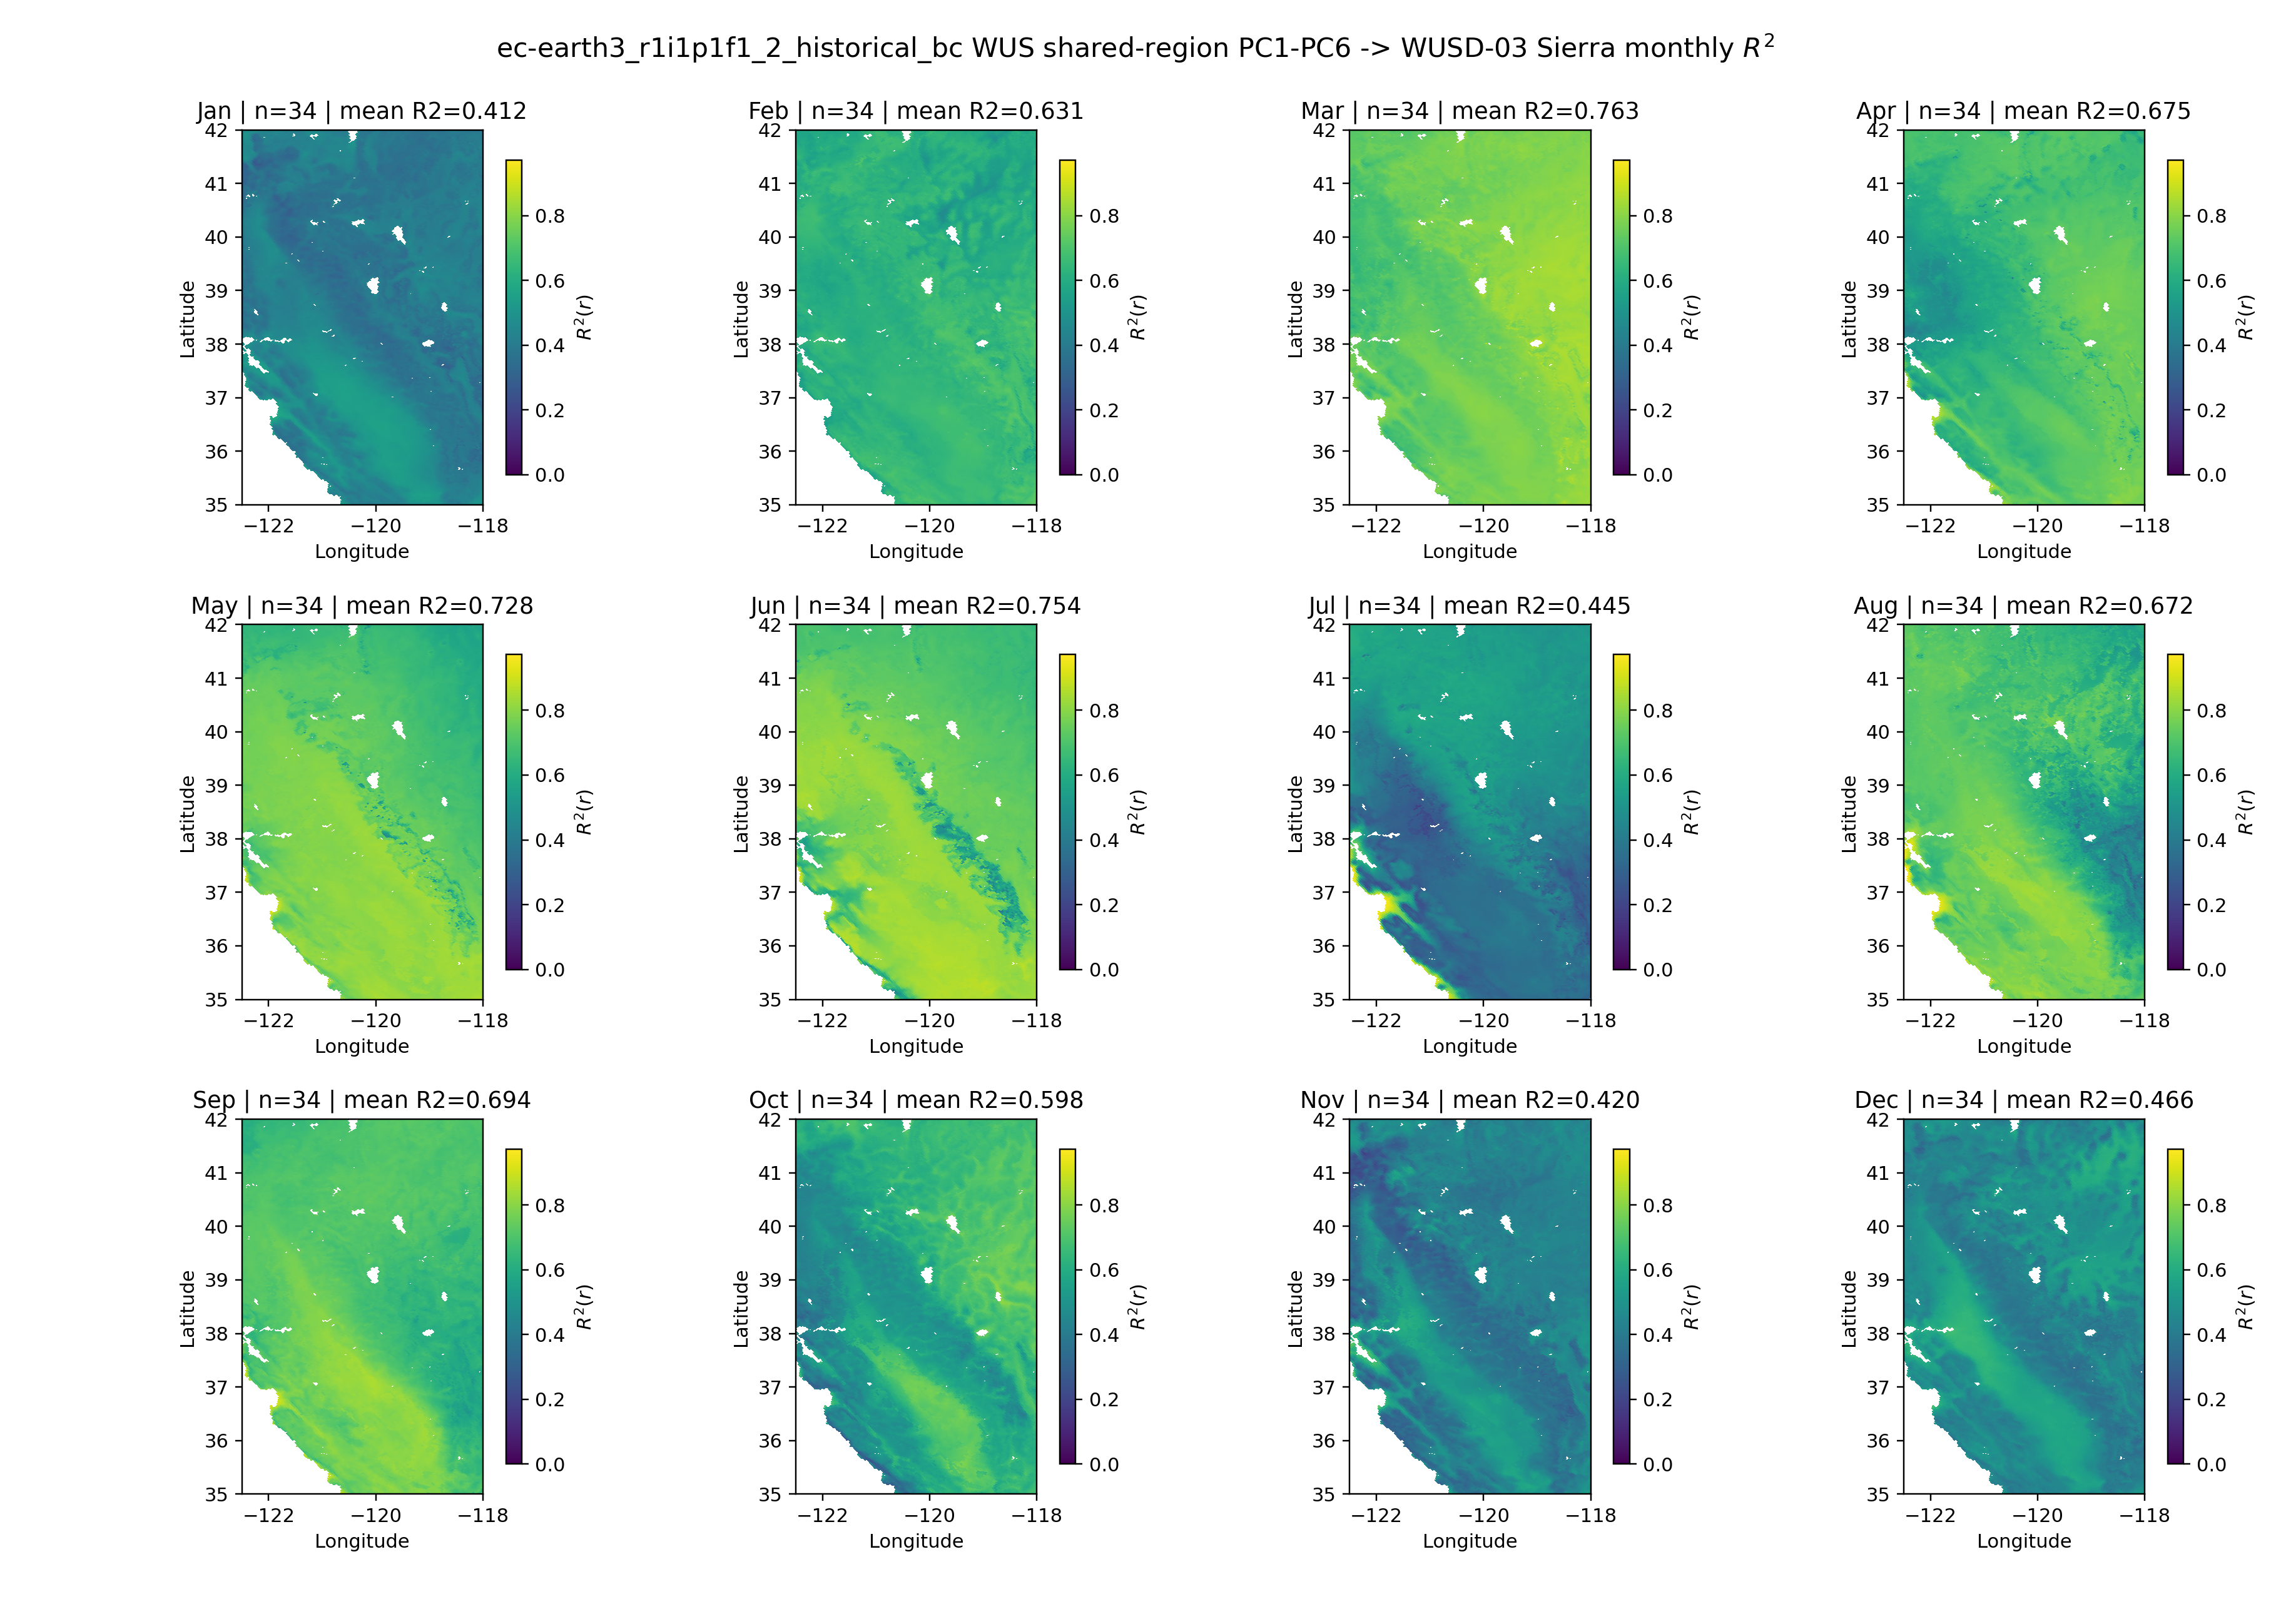
\includegraphics[width=0.88\linewidth]{../figures/wusd3_sharedregion_pc_t2m_level2_pc1to6_monthly_r2_maps.png}
\caption{Monthly six-PC $R^2(r)$ maps over the Sierra evaluation region using WUSD-03 SST
projected onto the shared-region COBE2 EOF basis. WUSD-03 SST anomalies are first projected onto
the COBE2 EOFs computed only over the WUSD-03 d01 SST coverage region. The resulting projected
scores are standardized and then used as predictors for WUSD-03 Sierra T2m anomalies. Each panel
is fit using only samples from that calendar month, following the same Level-2 monthly OLS
procedure used for the observational analysis. Source generating script:
\texttt{scripts/run\_cobe2\_sharedregion\_wusd3\_sierra\_t2m\_diagnostics.py}.}
\label{fig:wusd3_sharedregion_monthly_r2_maps}
\end{figure}



\section{COBE2 SST--Sierra SWE LOD Setup}
\label{sec:cobe2_swe_lod}

\subsection{Target: April 1 Sierra SWE}
\label{subsec:apr1_sierra_swe_target}

The target dataset is the UCLA WUS SWE product:
\begin{quote}
\path{WUS_UCLA_SR_v01_ALL_0_agg_16_WY{water_year}_SD_SWE_SCA_POST.nc}
\end{quote}
with source directory
\begin{quote}
\path{/global/cfs/projectdirs/m3522/datalake/UCLA_WUS_SNOWv1}
\end{quote}
The raw SWE variable is \texttt{SWE\_Post}, with units of meters and dimensions
\begin{equation}
(\mathrm{time}, \mathrm{Stats}, \mathrm{Latitude}, \mathrm{Longitude}).
\end{equation}
We use the mean SWE field, corresponding to \texttt{Stats}=0.

Let $SWE_i(d,y)$ denote the UCLA SWE value at grid cell $i$, date $d$, and water year $y$.
For each water year, we extract the April 1 SWE field:
\begin{equation}
SWE_i^{\mathrm{Apr1}}(y)
=
SWE_i(d=\mathrm{April\ 1\ of\ WY}\ y).
\label{eq:swe_apr1_grid}
\end{equation}

We then compute the Sierra-area-averaged April 1 SWE:
\begin{equation}
SWE_{\mathrm{Sierra}}^{\mathrm{Apr1}}(y)
=
\frac{
\sum_{i \in \Omega_{\mathrm{Sierra}}}
f_i A_i SWE_i^{\mathrm{Apr1}}(y)
}{
\sum_{i \in \Omega_{\mathrm{Sierra}}}
f_i A_i
}.
\label{eq:swe_apr1_area_average}
\end{equation}
Here $\Omega_{\mathrm{Sierra}}$ is the Sierra region, $f_i$ is the fractional Sierra mask value for
grid cell $i$, and $A_i$ is the physical grid-cell area. The Sierra region follows the current repo
definition:
\begin{equation}
35^\circ\mathrm{N} \leq \phi \leq 42^\circ\mathrm{N},
\qquad
122.5^\circ\mathrm{W} \leq \lambda \leq 118^\circ\mathrm{W}.
\end{equation}

Using all available UCLA water years gives one scalar target value per water year:
\begin{equation}
SWE_{\mathrm{Sierra}}^{\mathrm{Apr1}}(y),
\qquad
y = 1985,\ldots,2021.
\end{equation}
Therefore, the raw target vector has dimension
\begin{equation}
SWE_{\mathrm{Sierra}}^{\mathrm{Apr1}} \in \mathbb{R}^{37}.
\label{eq:swe_target_raw_dim}
\end{equation}

\subsection{April 1 SWE Anomaly and Standardization}
\label{subsec:apr1_swe_anomaly_standardization}

To construct the LOD target, we remove the April 1 climatological mean across the 37 water years:
\begin{equation}
\overline{SWE_{\mathrm{Sierra}}^{\mathrm{Apr1}}}
=
\frac{1}{37}
\sum_{y=1985}^{2021}
SWE_{\mathrm{Sierra}}^{\mathrm{Apr1}}(y).
\label{eq:swe_apr1_climatology}
\end{equation}
The April 1 SWE anomaly is then
\begin{equation}
SWE_{\mathrm{Sierra}}^{\mathrm{Apr1}\prime}(y)
=
SWE_{\mathrm{Sierra}}^{\mathrm{Apr1}}(y)
-
\overline{SWE_{\mathrm{Sierra}}^{\mathrm{Apr1}}}.
\label{eq:swe_apr1_anomaly}
\end{equation}
This anomaly vector still contains one sample per water year:
\begin{equation}
SWE_{\mathrm{Sierra}}^{\mathrm{Apr1}\prime} \in \mathbb{R}^{37}.
\end{equation}

Finally, the anomaly target is standardized before the LOD search:
\begin{equation}
\widetilde{SWE_{\mathrm{Sierra}}^{\mathrm{Apr1}}}(y)
=
\frac{
SWE_{\mathrm{Sierra}}^{\mathrm{Apr1}\prime}(y)
}{
\sigma_{SWE}
},
\label{eq:swe_apr1_standardized}
\end{equation}
where
\begin{equation}
\sigma_{SWE}
=
\sqrt{
\frac{1}{36}
\sum_{y=1985}^{2021}
\left[
SWE_{\mathrm{Sierra}}^{\mathrm{Apr1}\prime}(y)
\right]^2
}.
\label{eq:swe_apr1_std}
\end{equation}
The final standardized target used by LOD is dimensionless and has dimension
\begin{equation}
\widetilde{y}
=
\widetilde{SWE}{\mathrm{Sierra}}^{\mathrm{Apr1}}
\in \mathbb{R}^{37}.
\label{eq:lod_target_dim}
\end{equation}

\subsection{Predictor: COBE2 Monthly SST Anomalies}
\label{subsec:cobe2_sst_lod_predictor}

The predictor dataset is monthly COBE2 SST:
\begin{quote}
\path{/global/cfs/projectdirs/m3522/datalake/COBE2/sst.mon.mean.nc}
\end{quote}
Let $\sst(\lambda,\phi,t)$ denote monthly mean SST at longitude $\lambda$, latitude $\phi$, and
calendar month $t$. For this LOD experiment, COBE2 SST is restricted to the Pacific predictor
domain
\begin{equation}
-10^\circ \leq \phi \leq 60^\circ,
\qquad
120^\circ \leq \lambda \leq 280^\circ,
\label{eq:cobe2_sst_lod_pacific_domain}
\end{equation}
where longitude is expressed in $0..360$ coordinates. Only valid ocean grid cells inside this
Pacific domain are retained. Land and missing SST cells remain masked and are excluded from the
candidate predictor pool.

For each water year $y$, the SST predictors are taken from September through March:
\begin{equation}
m \in
{\mathrm{Sep}, \mathrm{Oct}, \mathrm{Nov}, \mathrm{Dec}, \mathrm{Jan}, \mathrm{Feb}, \mathrm{Mar}}.
\end{equation}
The water-year alignment is
\begin{equation}
\mathrm{WY}; y:
\quad
\mathrm{Sep}(y-1),\ \mathrm{Oct}(y-1),\ \mathrm{Nov}(y-1),\ \mathrm{Dec}(y-1),
\ \mathrm{Jan}(y),\ \mathrm{Feb}(y),\ \mathrm{Mar}(y).
\label{eq:sst_wy_alignment}
\end{equation}
For example, the WY1985 April 1 SWE target is paired with COBE2 SST from September 1984 through
March 1985.

For each lag month $m$, we compute a month-specific SST climatology over the 37 aligned water-year
samples:
\begin{equation}
\overline{\sst}(\lambda,\phi,m)
=
\frac{1}{37}
\sum_{y=1985}^{2021}
\sst(\lambda,\phi,m,y),
\label{eq:sst_lod_monthly_climatology}
\end{equation}
where $\sst(\lambda,\phi,m,y)$ denotes the SST value from lag month $m$ assigned to water year $y$.
The SST anomaly is
\begin{equation}
\sst'(\lambda,\phi,m,y)
=
\sst(\lambda,\phi,m,y)
-
\overline{\sst}(\lambda,\phi,m).
\label{eq:sst_lod_anomaly}
\end{equation}

After subsetting to Eq.~\eqref{eq:cobe2_sst_lod_pacific_domain}, the COBE2 grid used by the script
contains $70$ latitude points and $160$ longitude points, so the unmasked Pacific box has
$70 \times 160 = 11{,}200$ grid cells. Among those, $9{,}149$ cells are valid ocean points. In the
current run, the same $9{,}149$ valid ocean cells are available in each lag month from September
through March. Therefore the anomaly array can be viewed as
\begin{equation}
\sst' \in \mathbb{R}^{37 \times 7 \times 9149},
\label{eq:sst_lod_ocean_only_dim}
\end{equation}
with axes water year, lag month, and ocean-cell index.

For LOD, the lag-month axis and ocean-cell axis are combined into one predictor-column axis:
\begin{equation}
X \in \mathbb{R}^{37 \times P},
\qquad
P = 7N_{\mathrm{ocean}} = 7 \times 9149 = 64{,}043.
\label{eq:sst_lod_flattened_dim}
\end{equation}
The rows of $X$ are water years. The columns of $X$ are individual SST predictor time series. Each
column corresponds to one specific lag month and one specific COBE2 ocean grid cell.

To make the column indexing explicit, consider a small example with only three lag months and four
valid ocean cells. In that toy case, the predictor matrix has
\[
P = 3 \times 4 = 12.
\]
The ordering is
\begin{equation}
\begin{aligned}
p=1,2,3,4 &\longrightarrow (\mathrm{Sep},\mathrm{cell}1\text{--}4),\\
p=5,6,7,8 &\longrightarrow (\mathrm{Oct},\mathrm{cell}1\text{--}4),\\
p=9,10,11,12 &\longrightarrow (\mathrm{Mar},\mathrm{cell}1\text{--}4).
\end{aligned}
\label{eq:lod_flattening_example_table}
\end{equation}
Thus the first predictor row would be
\begin{equation}
\begin{aligned}
X_{1,:} = \bigl[
&X(\mathrm{Sep1984},\mathrm{cell}1),\ldots,X(\mathrm{Sep1984},\mathrm{cell}4),\\
&X(\mathrm{Oct1984},\mathrm{cell}1),\ldots,X(\mathrm{Oct1984},\mathrm{cell}4),\\
&X(\mathrm{Mar1985},\mathrm{cell}1),\ldots,X(\mathrm{Mar1985},\mathrm{cell}4)
\bigr].
\end{aligned}
\label{eq:lod_flattening_example_row}
\end{equation}

In the real experiment, the same ordering is used with seven lag months:
\[
\mathrm{Sep},\mathrm{Oct},\mathrm{Nov},\mathrm{Dec},\mathrm{Jan},\mathrm{Feb},\mathrm{Mar}.
\]
If $l$ is the lag-month index and $i$ is the ocean-cell index, then the predictor-column index is
\begin{equation}
p=(l-1)N_{\mathrm{ocean}}+i.
\label{eq:lod_flattening_column_index}
\end{equation}
Therefore $X_{n,p}$ is one scalar SST predictor value for water-year row $n$ and predictor
column $p$. The column vector $X_{:,p}$ is the 37-year SST time series that LOD compares against
the 37-year April 1 Sierra SWE target.

Each valid SST predictor column is standardized across the 37 water-year samples:
\begin{equation}
\widetilde{X}_{n,p}
=
\frac{
X_{n,p} - \overline{X}_p
}{
\sigma_p
},
\label{eq:sst_candidate_standardized}
\end{equation}
where
\begin{equation}
\overline{X}_p
=
\frac{1}{37}
\sum_{n=1}^{37}
X_{n,p},
\qquad
\sigma_p
=
\sqrt{
\frac{1}{36}
\sum_{n=1}^{37}
\left[X_{n,p}-\overline{X}_p\right]^2
}.
\label{eq:sst_candidate_mean_std}
\end{equation}
The standardized predictor matrix therefore has dimension
\begin{equation}
\widetilde{X} \in \mathbb{R}^{37 \times 64{,}043}.
\label{eq:sst_standardized_predictor_dim}
\end{equation}


\subsection{LOD Formulation for SST Predictors and April 1 SWE}
\label{subsec:cobe2_swe_lod_formulation}

The LOD target is the standardized April 1 Sierra SWE anomaly:
\begin{equation}
\widetilde{y}(n)
=
\widetilde{SWE}_{\mathrm{Sierra}}^{\mathrm{Apr1}}(n),
\qquad
n=1,\ldots,37.
\label{eq:lod_target_definition}
\end{equation}
Here $n$ indexes the 37 water-year samples, corresponding to WY1985--WY2021.

The predictor matrix is the standardized COBE2 SST anomaly matrix:
\begin{equation}
\widetilde{X} \in \mathbb{R}^{37\times P},
\qquad
P = 64{,}043,
\label{eq:lod_predictor_dimension}
\end{equation}
where the 37 rows are water years and each column is one lagged SST predictor time series from the
Pacific domain defined in Eq.~\eqref{eq:cobe2_sst_lod_pacific_domain}. The seven lag months are
September, October, November, December, January, February, and March. The quantity
$N_{\mathrm{ocean}}$ is the number of valid COBE2 ocean grid cells in the selected Pacific domain.

We use $p=1,\ldots,P$ to index the predictor columns. Each column $p$ corresponds to one
specific lag month and one specific ocean grid cell:
\begin{equation}
p \longrightarrow (m_p,\phi_p,\lambda_p),
\label{eq:lod_predictor_column_mapping}
\end{equation}
where $m_p$ is the lag month and $(\phi_p,\lambda_p)$ is the COBE2 ocean grid-cell location.
The matrix entry
\begin{equation}
\widetilde{X}_{n,p}
\in \mathbb{R}
\label{eq:lod_predictor_entry}
\end{equation}
is therefore one scalar value: the standardized SST anomaly for water-year sample $n$ and
predictor column $p$. The column vector $\widetilde{X}_{:,p}\in\mathbb{R}^{37}$ is the full
37-year SST predictor time series used in the LOD search.

LOD starts from the full standardized SWE target as the initial residual:
\begin{equation}
r_0(n)=\widetilde{y}(n).
\label{eq:lod_initial_residual}
\end{equation}
At mode $k$, the algorithm searches over all SST predictor columns and selects the one with the
largest absolute correlation with the current residual:
\begin{equation}
p_k
=
\arg\max_{p=1,\ldots,P}
\left|
\mathrm{corr}\left(r_{k-1},\widetilde{X}_{:,p}\right)
\right|.
\label{eq:lod_mode_selection}
\end{equation}
The selected SST time series is
\begin{equation}
u_k(n)=\widetilde{X}_{n,p_k}.
\label{eq:lod_selected_candidate}
\end{equation}

To make each newly selected mode independent of the previously retained modes, $u_k$ is
orthogonalized against $M_1,\ldots,M_{k-1}$:
\begin{equation}
\widehat{M}_k(n)
=
u_k(n)
-
\sum_{j=1}^{k-1}
\frac{
\sum_{n=1}^{37} u_k(n)M_j(n)
}{
\sum_{n=1}^{37} M_j(n)^2
}
M_j(n).
\label{eq:lod_orthogonalization}
\end{equation}
For the first mode, the summation is empty, so
\begin{equation}
\widehat{M}_1(n)=u_1(n).
\end{equation}
The orthogonalized mode is then standardized:
\begin{equation}
M_k(n)
=
\frac{
\widehat{M}_k(n)-\overline{\widehat{M}_k}
}{
\sigma_{\widehat{M}_k}
},
\label{eq:lod_mode_standardization}
\end{equation}
where
\begin{equation}
\overline{\widehat{M}_k}
=
\frac{1}{37}
\sum_{n=1}^{37}
\widehat{M}_k(n),
\qquad
\sigma_{\widehat{M}_k}
=
\sqrt{
\frac{1}{36}
\sum_{n=1}^{37}
\left[
\widehat{M}_k(n)-\overline{\widehat{M}_k}
\right]^2
}.
\label{eq:lod_mode_mean_std}
\end{equation}

The contribution of mode $k$ is obtained by projecting the current residual onto the standardized
mode $M_k$:
\begin{equation}
\beta_k
=
\frac{
\sum_{n=1}^{37} M_k(n)r_{k-1}(n)
}{
\sum{n=1}^{37} M_k(n)^2
},
\qquad
\widehat{r}_{k-1,k}(n)=\beta_k M_k(n).
\label{eq:lod_projection}
\end{equation}
The residual is updated by subtracting this fitted component:
\begin{equation}
r_k(n)
=
r_{k-1}(n)-\beta_k M_k(n).
\label{eq:lod_residual_update}
\end{equation}

After $k$ modes, the reconstructed standardized April 1 SWE anomaly is
\begin{equation}
\widehat{y}_k(n)
=
\sum_{j=1}^{k}
\beta_j M_j(n),
\label{eq:lod_reconstruction}
\end{equation}
and the remaining residual is
\begin{equation}
r_k(n)
=
\widetilde{y}(n)-\widehat{y}_k(n).
\label{eq:lod_remaining_residual}
\end{equation}

The cumulative explained variance after $k$ modes is
\begin{equation}
R_k^2
=
1
-
\frac{
\sum_{n=1}^{37} r_k(n)^2
}{
\sum_{n=1}^{37} \widetilde{y}(n)^2
}.
\label{eq:lod_cumulative_r2}
\end{equation}
The marginal gain from adding mode $k$ is
\begin{equation}
\Delta R_k^2
=
R_k^2-R_{k-1}^2,
\qquad
R_0^2=0.
\label{eq:lod_incremental_r2}
\end{equation}

The diagnostic uses
\begin{equation}
K_{\max}=6
\label{eq:lod_kmax}
\end{equation}
as the maximum search depth. This is only a diagnostic ceiling, not the assumed number of useful
modes. After each mode, the extraction stops if the new mode adds too little explained variance:
\begin{equation}
\Delta R_k^2 < 0.02,
\label{eq:lod_stop_delta_r2}
\end{equation}
or if the selected SST predictor has weak correlation with the current residual:
\begin{equation}
\left|
\mathrm{corr}\left(r_{k-1},\widetilde{X}_{:,p_k}\right)
\right| < 0.2.
\label{eq:lod_stop_corr}
\end{equation}
The selected number of retained modes is therefore
\begin{equation}
K^*
=
\min\left\{
k \leq 6 :
\Delta R_k^2 < 0.02
\ \mathrm{or}\
\left|
\mathrm{corr}\left(r_{k-1},\widetilde{X}_{:,p_k}\right)
\right| < 0.2
\right\}.
\label{eq:lod_kstar}
\end{equation}
If neither stopping condition is reached by six modes, the diagnostic stops at $K_{\max}=6$.

For each retained mode, the selected predictor column $p_k$ is mapped back to its physical SST
lag month and grid location:
\begin{equation}
p_k \longrightarrow (m_k,\phi_k,\lambda_k).
\label{eq:lod_output_candidate}
\end{equation}
The output table records $m_k$, $\phi_k$, $\lambda_k$, the selected residual correlation,
$\beta_k$, $R_k^2$, and $\Delta R_k^2$. Each selected mode therefore identifies one
Pacific-domain COBE2 SST time series that explains part of the remaining April 1 Sierra SWE
anomaly residual.

\subsection{Current Pacific-Domain COBE2--Sierra SWE LOD Diagnostic}
\label{subsec:cobe2_swe_lod_results}

The Pacific-only LOD diagnostic was run with the standardized April 1 Sierra SWE target for water
years 1985--2021 and COBE2 monthly SST anomalies from September through March over the domain in
Eq.~\eqref{eq:cobe2_sst_lod_pacific_domain}. The produced artifacts are
\begin{quote}
\small
\path{/pscratch/sd/h/hyvchen/Snow-Predication-at-Sierra/artifacts/}\\
\path{cobe2_sierra_swe_lod_setup/lod_analysis/}
\path{cobe2_sierra_swe_lod_summary.json}\\
\path{cobe2_sierra_swe_lod_modes.csv}\\
\path{cobe2_sierra_swe_lod_diagnostics.nc}
\end{quote}

The standardized predictor matrix contained
\begin{equation}
\widetilde{X}\in\mathbb{R}^{37\times 64{,}043},
\end{equation}
with $9{,}149$ valid Pacific ocean cells in each of the seven lag months. The run completed in
approximately $5.49$ seconds with a reported peak memory of about $206$ MB. None of the stopping
criteria was triggered before the sixth mode, so the diagnostic reached the prescribed maximum
depth $K_{\max}=6$. The cumulative explained variance after each retained mode was
\begin{equation}
R_1^2=0.2394,\quad
R_2^2=0.3998,\quad
R_3^2=0.5518,\quad
R_4^2=0.6360,\quad
R_5^2=0.7167,\quad
R_6^2=0.7863.
\label{eq:cobe2_swe_lod_r2_values}
\end{equation}

\begin{table}[h]
\centering
\caption{Retained Pacific-domain COBE2 SST predictors in the current Sierra SWE LOD diagnostic.
Longitudes are reported in $0..360$ coordinates.}
\begin{tabular}{ccccccc}
\hline
Mode & Lag & Lat. & Lon. & Corr. & $\Delta R_k^2$ & $R_k^2$ \\
\hline
1 & Jan & $-9.5^\circ$ & $133.5^\circ$ & $-0.4893$ & $0.2394$ & $0.2394$ \\
2 & Oct & $0.5^\circ$ & $136.5^\circ$ & $0.4464$ & $0.1605$ & $0.3998$ \\
3 & Sep & $-7.5^\circ$ & $156.5^\circ$ & $-0.4610$ & $0.1519$ & $0.5518$ \\
4 & Sep & $27.5^\circ$ & $275.5^\circ$ & $-0.4284$ & $0.0843$ & $0.6360$ \\
5 & Sep & $42.5^\circ$ & $195.5^\circ$ & $0.4568$ & $0.0807$ & $0.7167$ \\
6 & Jan & $50.5^\circ$ & $147.5^\circ$ & $0.4655$ & $0.0696$ & $0.7863$ \\
\hline
\end{tabular}
\label{tab:cobe2_swe_lod_modes}
\end{table}

\paragraph{ERA5 cross-dataset LOD status note.}
An ERA5-SST version of the same Sierra SWE LOD setup was run with the identical April 1 Sierra SWE
target, the same September--March water-year alignment, the same Pacific predictor domain, and the
same stopping criteria as the COBE2 diagnostic. No reusable processed ERA5 Pacific monthly-SST
anomaly product was found under the searched artifact trees, so the predictor was created anew from
raw hourly ERA5 \texttt{SSTK} files for September 1984 through March 2021. The new processed
predictor product is
\begin{quote}
\small
\path{/pscratch/sd/h/hyvchen/Snow-Predication-at-Sierra/artifacts/}\\
\path{era5_sierra_swe_lod_setup/predictors/}\\
\path{era5_pacific_sst_monthly_anomaly_wy1985_2021_sep1984_mar2021.nc}
\end{quote}
and the ERA5 LOD artifacts are
\begin{quote}
\small
\path{/pscratch/sd/h/hyvchen/Snow-Predication-at-Sierra/artifacts/}\\
\path{era5_sierra_swe_lod_setup/lod_analysis/era5_sierra_swe_lod_summary.json}\\
\path{era5_sierra_swe_lod_setup/lod_analysis/era5_sierra_swe_lod_modes.csv}\\
\path{era5_sierra_swe_lod_setup/lod_analysis/era5_sierra_swe_lod_diagnostics.nc}
\end{quote}
with the cross-dataset comparison written to
\begin{quote}
\small
\path{/pscratch/sd/h/hyvchen/Snow-Predication-at-Sierra/artifacts/}\\
\path{cobe2_era5_sst_sierra_swe_lod_comparison/cobe2_era5_lod_mode_comparison.csv}\\
\path{cobe2_era5_sst_sierra_swe_lod_comparison/cobe2_era5_lod_comparison_summary.json.}
\end{quote}
The final standardized ERA5 predictor matrix is
\begin{equation}
\widetilde{X}_{\mathrm{ERA5}}\in\mathbb{R}^{37\times 1{,}023{,}281},
\end{equation}
corresponding to $146{,}183$ shared valid Pacific ocean cells across the seven lag months. The
retained ERA5 modes are
\begin{center}
\begin{tabular}{ccccccc}
\hline
Mode & Lag & Lat. & Lon. & Corr. & $\Delta R_k^2$ & $R_k^2$ \\
\hline
1 & Sep & $35.25^\circ$ & $125.75^\circ$ & $0.5766$ & $0.3324$ & $0.3324$ \\
2 & Feb & $-8.75^\circ$ & $277.5^\circ$ & $0.5494$ & $0.2016$ & $0.5341$ \\
3 & Sep & $55.5^\circ$ & $244.75^\circ$ & $-0.5601$ & $0.1492$ & $0.6833$ \\
4 & Feb & $23.75^\circ$ & $154.25^\circ$ & $-0.5758$ & $0.1080$ & $0.7913$ \\
5 & Sep & $21.25^\circ$ & $269.5^\circ$ & $0.5959$ & $0.0810$ & $0.8723$ \\
6 & Dec & $56.75^\circ$ & $146.5^\circ$ & $-0.5600$ & $0.0463$ & $0.9187$ \\
\hline
\end{tabular}
\end{center}
The cumulative ERA5 curve is therefore steeper than the COBE2 curve:
\begin{equation}
R_{k,\mathrm{ERA5}}^2=(0.3324,\ 0.5341,\ 0.6833,\ 0.7913,\ 0.8723,\ 0.9187),
\end{equation}
compared with the COBE2 values in Eq.~\eqref{eq:cobe2_swe_lod_r2_values}. However, the cross-dataset
comparison does \emph{not} show matching leading modes in similar broad Pacific regions. Under the
coarse broad-region binning used in the comparison script, ERA5 and COBE2 agree on none of the
first three mode regions, and only the sixth mode lands in the same broad midlatitude western
Pacific sector. The first three modes in both datasets are more stable than later modes in the
sense that their mean $\Delta R_k^2$ exceeds the mean $\Delta R_k^2$ of later retained modes, but
that stability alone is not enough for the paper-style cross-dataset robustness test. The current
evidence therefore does not support retaining the ERA5 and COBE2 \emph{leading} modes as shared
robust SST predictors in the same way as the paper's cross-dataset logic; at present, the leading
structures are dataset-dependent, with only a later midlatitude western Pacific mode showing broad
agreement.


\section{Understanding SWE and SST}

Our overall goal is to understand and reduce the SST predictor space for Sierra SWE prediction.
The target is April 1 SWE over the Sierra Nevada, possibly separated into northern, middle, and
southern Sierra subregions. The candidate predictor is monthly SST anomaly from September through
March over the broad Pacific domain, defined here as $10^\circ\mathrm{S}$--$60^\circ\mathrm{N}$
and $120^\circ\mathrm{E}$--$280^\circ\mathrm{E}$ in $0..360$ longitude convention. Because only
about 37 water years are available, the full SST field cannot be used directly as model input
without severe overfitting. Therefore, we first need to identify which parts of the SST information
are most relevant to SWE before training the final prediction model.

We will pursue two complementary directions.

The first direction is a known-climate-mode baseline. In this approach, we reduce SST using established oceanic modes of variability, such as broad Pacific SST EOF-PC modes, Niño 3.4, and AMV/AMO. These predictors are constructed from physically motivated ocean domains using either area averaging or EOF/PCA-based projection. Following the logic of the recent climate-mode predictability paper, we will test how much April 1 SWE variability can be predicted from these climate-mode predictor time series under leave-one-year-out cross-validation. This direction asks whether known large-scale SST variability patterns contain useful predictive information for Sierra SWE.

The second direction is direct SST-field discovery. In this approach, we do not assume that the SWE-relevant SST signal must align with predefined climate modes or EOF patterns. Instead, we start from the full Pacific SST anomaly field from September through March and ask which months, locations, or coherent SST regions are most strongly and stably related to April 1 SWE. This direction is needed because EOF-based climate modes may compress the SST field too strongly and may miss smaller or more regional SST signals that are still relevant to Sierra SWE.


\subsection{Known-Climate-Mode SWE Baseline}
\label{subsec:swe_known_climate_mode_baseline}

\begin{figure}[h]
\centering
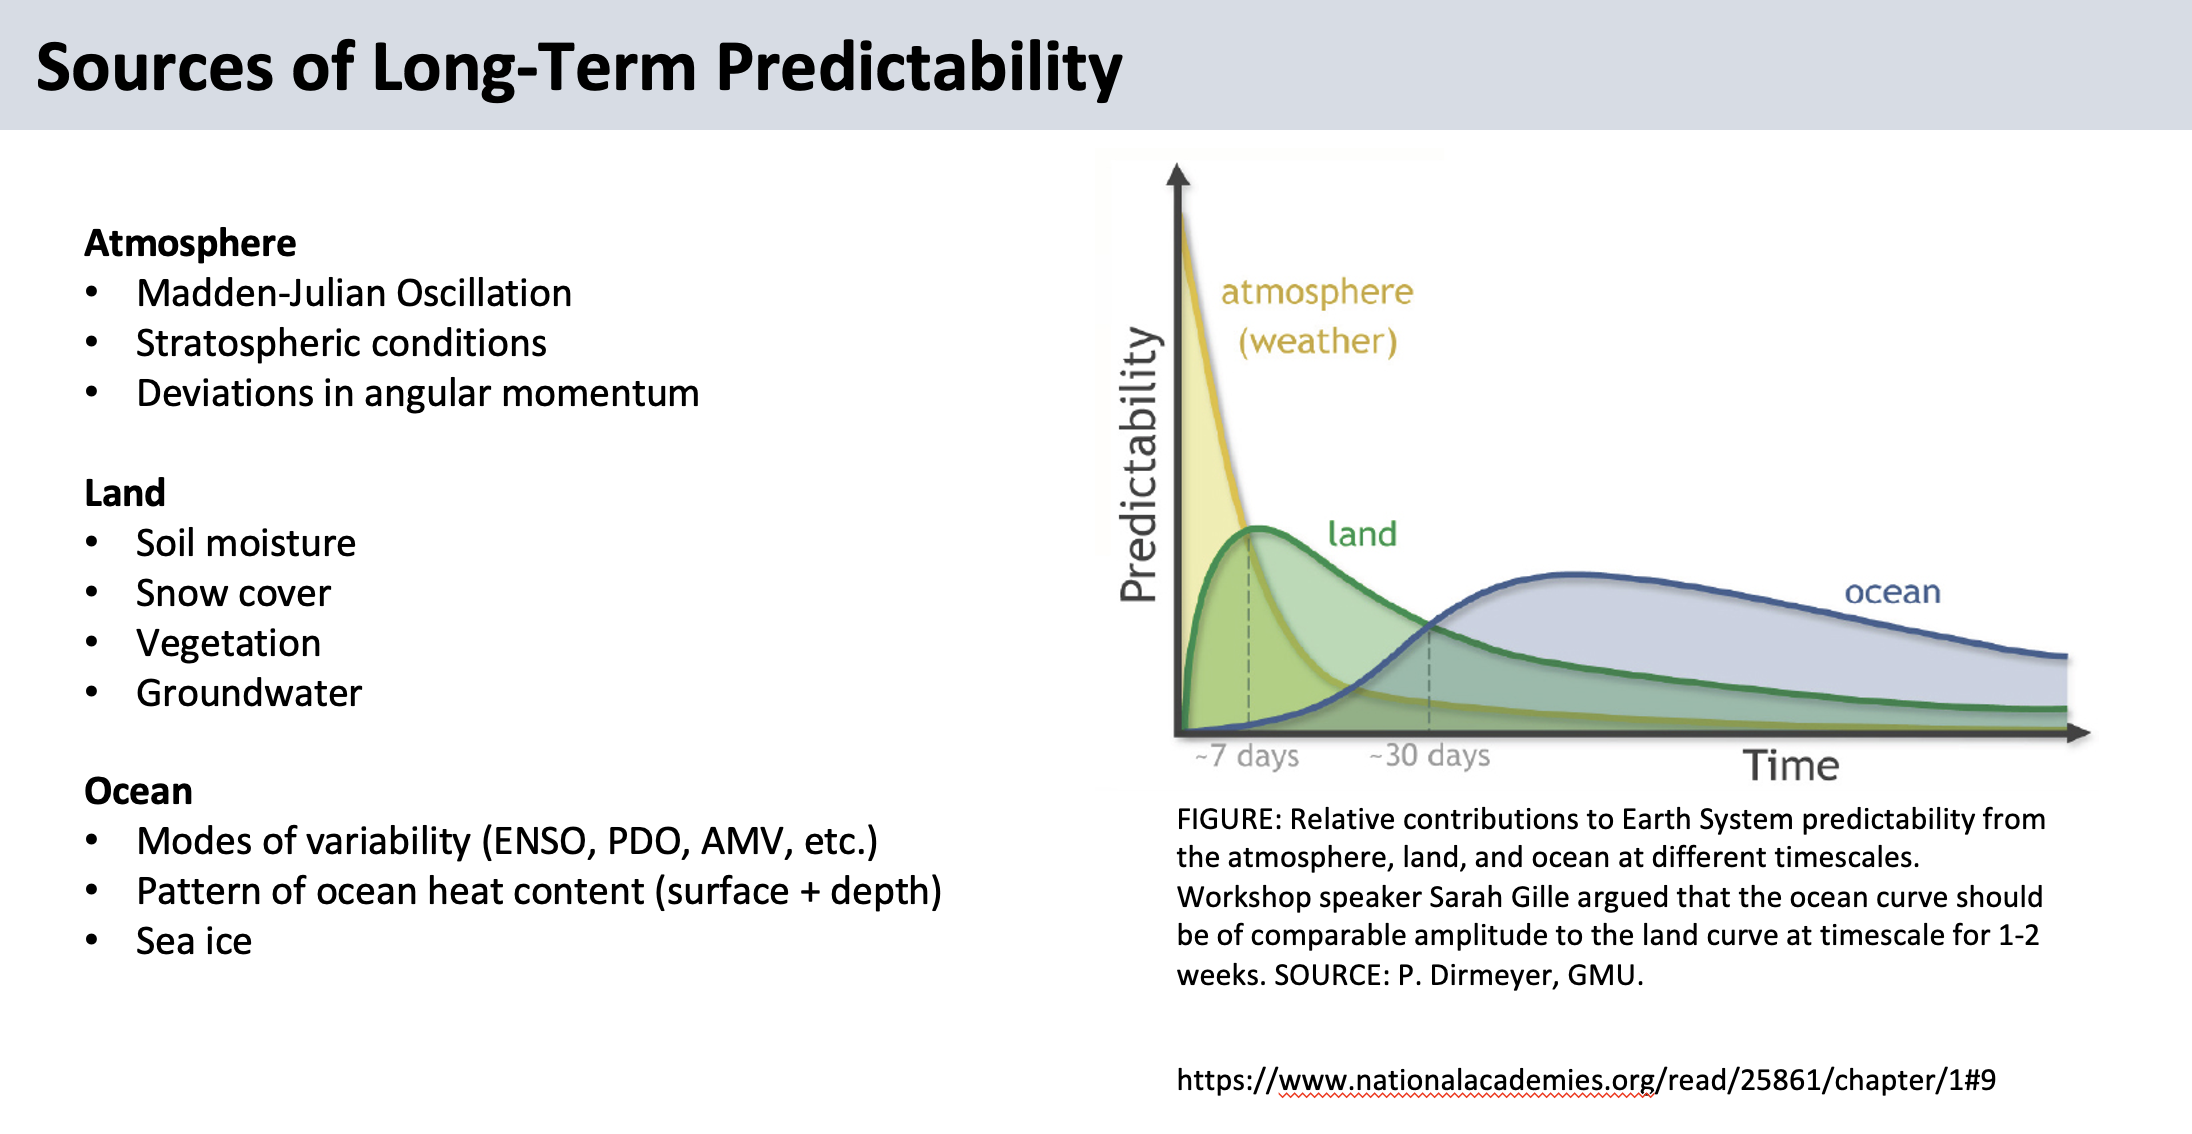
\includegraphics[width=0.96\linewidth]{../figures/souces_of_long_term_predictability.png}
\caption{Broader sources of long-term predictability relevant to Sierra SWE, spanning the
atmosphere, land, and ocean. In the current baseline workflow, we start from the ocean side first
by testing ocean modes of variability before adding later atmospheric or land-based predictor
groups.}
\label{fig:sources_of_long_term_predictability}
\end{figure}

The reference paper: \href{https://doi.org/10.1038/s43247-024-01594-2}{Higher-order internal modes of variability imprinted in year-to-year California streamflow changes}.
The goal of the latest session is to introduce the first baseline direction for the Sierra SWE
prediction project: a known-climate-mode baseline. 


The initial ocean-mode baseline is restricted to three predictor groups: COBE2
broad Pacific SST EOF-PC modes, the Ni\~no 3.4 SST index, and AMV/AMO North Atlantic SST EOF-PC
modes. 

The existing COBE2 Pacific SST EOF-PC products should be described as broad Pacific SST modes over
$10^\circ\mathrm{S}$--$60^\circ\mathrm{N}$ and $120^\circ\mathrm{E}$--$280^\circ\mathrm{E}$ in
$0..360$ longitude, equivalently $120^\circ\mathrm{E}$--$80^\circ\mathrm{W}$. They should not be
labeled directly as ENSO or PDO. Instead, these broad Pacific EOF-PC modes may contain basin-wide
warming, ENSO-like variability, and PDO-like variability among modes 1--6, and those
interpretations should only be assigned after inspecting the EOF maps and comparing the PC time
series with known climate indices.

\begin{table}[h]
\centering
\small
\begin{tabular}{>{\raggedright\arraybackslash}p{0.14\linewidth}
                >{\raggedright\arraybackslash}p{0.08\linewidth}
                >{\raggedright\arraybackslash}p{0.20\linewidth}
                >{\raggedright\arraybackslash}p{0.20\linewidth}
                >{\raggedright\arraybackslash}p{0.24\linewidth}
                >{\raggedright\arraybackslash}p{0.10\linewidth}}
\toprule
Mode / index & Variable & Domain & Method & Expected predictor columns & Status \\
\midrule
COBE2 Pacific SST modes
& SST
& $10^\circ\mathrm{S}$--$60^\circ\mathrm{N}$, $120^\circ\mathrm{E}$--$280^\circ\mathrm{E}$ in $0..360$, equivalently $120^\circ\mathrm{E}$--$80^\circ\mathrm{W}$
& EOF1--EOF6 / PC1--PC6 from the existing COBE2 broad Pacific SST EOF workflow
& Sep--Mar Pacific SST PC1--PC6 values. These modes may contain basin-wide warming, ENSO-like variability, and PDO-like variability, but those interpretations should only be assigned after inspecting the EOF maps and PC correlations.
& Existing artifacts; reuse \\

Ni~no 3.4
& SST
& $5^\circ\mathrm{S}$--$5^\circ\mathrm{N}$, $190^\circ\mathrm{E}$--$240^\circ\mathrm{E}$ in $0..360$, equivalently $170^\circ\mathrm{W}$--$120^\circ\mathrm{W}$
& Area-weighted domain average of monthly SST anomalies
& \texttt{Nino34\_Sep}, \texttt{Nino34\_Oct}, \texttt{Nino34\_Nov}, \texttt{Nino34\_Dec}, \texttt{Nino34\_Jan}, \texttt{Nino34\_Feb}, \texttt{Nino34\_Mar}
& Generated \\

AMV / AMO
& SST
& $0^\circ$--$70^\circ\mathrm{N}$, $280^\circ\mathrm{E}$--$360^\circ\mathrm{E}$ in $0..360$, equivalently $80^\circ\mathrm{W}$--$0^\circ$
& Separate EOF1--EOF6 / PC1--PC6 analysis over the North Atlantic SST anomaly field; this does not reuse the Pacific EOF basis
& Sep--Mar AMV/AMO PC1--PC6 values
& Generated \\
\bottomrule
\end{tabular}
\caption{Ocean-side known-climate-mode baseline predictors for the Sierra SWE project. Exact artifact paths are listed below the table to keep the table readable.}
\label{tab:swe_known_climate_mode_baseline}
\end{table}

\paragraph{Artifact paths for Table~\ref{tab:swe_known_climate_mode_baseline}.}
The COBE2 Pacific SST EOF-PC products should be reused from the existing artifacts:
\begin{itemize}
    \item EOF/PC source: \path{artifacts/sst_pca/cobe2_global_monthly_climatology_anomaly/cobe2_global_monthly_clim_sst_eofs.nc}
    \item Existing EOF diagnostic figure: \path{artifacts/cobe2_pacific_sierra_t2m_level1_diagnostic/cobe2_pacific_sierra_cobe2_eofs_modes1to6.png}
    \item Existing Sep--Mar overlap PC file: \path{/pscratch/sd/h/hyvchen/Snow-Predication-at-Sierra/artifacts/cobe2_pacific_sierra_t2m_level2_pc1to6/cobe2_pacific_sierra_t2m_level2_pc1to6.nc}
    \item Run log: \path{artifacts/cobe2_pacific_sierra_t2m_level2_pc1to6/run.log}
\end{itemize}

The Ni~no 3.4 SST anomaly index has already been generated:
\begin{itemize}
    \item CSV table: \path{artifacts/swe_climate_mode_baseline/nino34/nino34_monthly_wy1985_2021_sep_mar.csv}
    \item NetCDF file: \path{artifacts/swe_climate_mode_baseline/nino34/nino34_monthly_wy1985_2021_sep_mar.nc}
    \item Summary metadata: \path{artifacts/swe_climate_mode_baseline/nino34/nino34_monthly_wy1985_2021_sep_mar_summary.json}
\end{itemize}

The AMV/AMO North Atlantic SST EOF-PC product has already been generated:
\begin{itemize}
    \item EOF/PC NetCDF file: \path{artifacts/swe_climate_mode_baseline/amv_amo/amv_amo_cobe2_north_atlantic_eofs_pc1to6.nc}
    \item Sep--Mar PC predictor table: \path{artifacts/swe_climate_mode_baseline/amv_amo/amv_amo_cobe2_north_atlantic_pc1to6_wy1985_2021_sep_mar.csv}
    \item Summary metadata: \path{artifacts/swe_climate_mode_baseline/amv_amo/amv_amo_cobe2_north_atlantic_pc1to6_summary.json}
    \item EOF diagnostic figure copied into the documentation figures directory: \path{figures/amv_amo_cobe2_north_atlantic_eofs_modes1to6.png}
    \item Run log: \path{artifacts/swe_climate_mode_baseline/amv_amo/run.log}
\end{itemize}

\paragraph{Clarification.}
For EOF-based predictors, the machine-learning input columns are the PC time series, not the EOF
maps. The EOF maps are used for physical interpretation. The COBE2 Pacific SST EOF-PC products are
broad Pacific SST modes; they may contain basin-wide warming, ENSO-like, and PDO-like structures,
but we should not assign those labels until the modes are inspected. AMV/AMO must be generated
from a separate North Atlantic SST EOF/PCA because the AMV/AMO domain is outside the Pacific EOF
domain.

\paragraph{AMV/AMO note.}
AMV/AMO is treated here as a North Atlantic SST variability predictor family. We use the label
AMV/AMO because AMV is the more neutral terminology, while AMO is the older ``oscillation''
terminology. In this baseline, the actual machine-learning predictor columns are the North
Atlantic SST PC time series, not the EOF maps. The EOF maps are retained only for physical
interpretation. EOF sign is arbitrary, so the sign of AMV/AMO PC1--PC6 should not be interpreted
without checking the EOF map and/or correlation with a reference AMV/AMO index, the visulization of the 6 modes are in Figure~\ref{fig:amv_amo_cobe2_north_atlantic_eofs_modes1to6}



\begin{figure}[h]
\centering
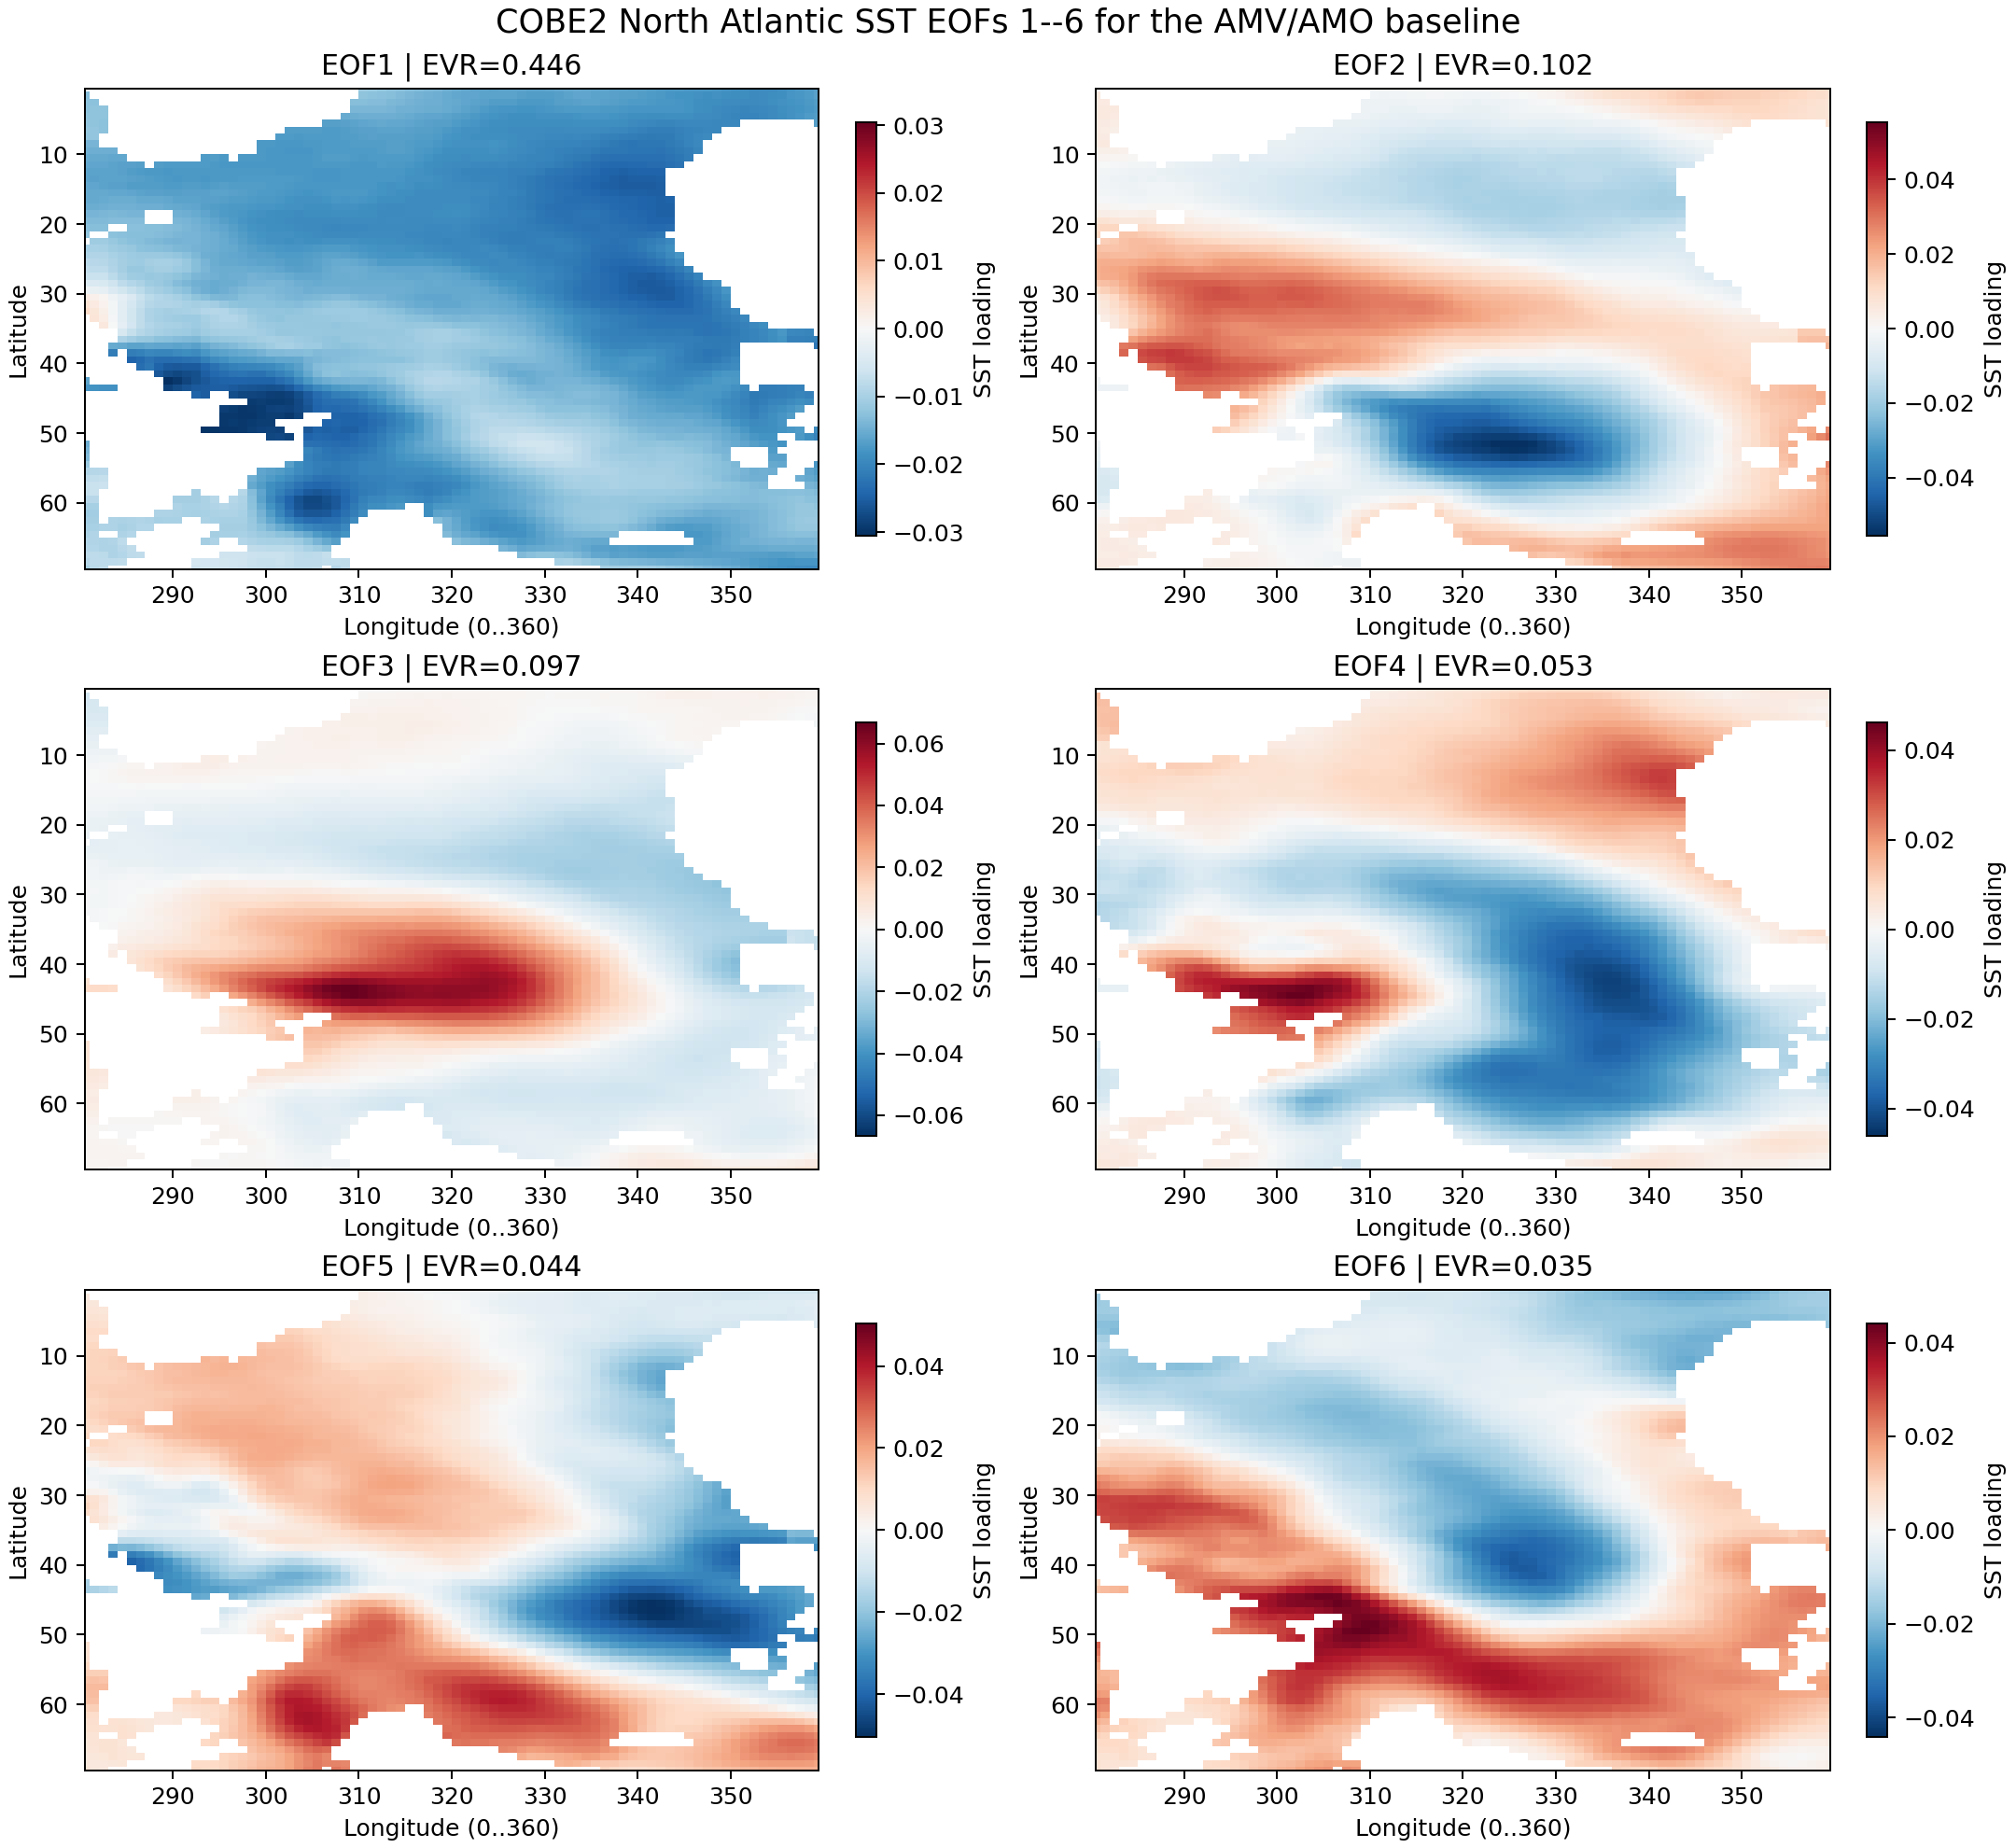
\includegraphics[width=0.92\linewidth]{../figures/amv_amo_cobe2_north_atlantic_eofs_modes1to6.png}
\caption{North Atlantic AMV/AMO baseline EOF diagnostic for COBE2 SST over $0^\circ$--$70^\circ\mathrm{N}$ and $280^\circ\mathrm{E}$--$360^\circ\mathrm{E}$ in the $0..360$ longitude convention. The panels show EOF modes 1--6 retained for the AMV/AMO predictor-family baseline.}
\label{fig:amv_amo_cobe2_north_atlantic_eofs_modes1to6}
\end{figure}


\subsubsection{Ocean-Mode-Only Predictability Test}
\label{subsubsec:ocean_mode_only_predictability_test}

After constructing the ocean-side known-climate-mode predictor table, the first prediction experiment
is an ocean-mode-only predictability test. The goal is to quantify how much April 1 Sierra SWE
variability can be predicted from the oceanic climate-mode predictors alone, without using any
same-year observed SWE state such as December 30 SWE. This experiment is intended to answer the
following question:

\begin{quote}
How much out-of-sample April 1 Sierra SWE predictability is contained in the ocean-mode predictor
set consisting of COBE2 Pacific SST PCs, Ni~no 3.4, and AMV/AMO North Atlantic SST PCs?
\end{quote}

The target variable is April 1 SWE. Because the Sierra Nevada is divided into northern, middle, and
southern subregions to avoid forcing one spatially averaged model onto regions with potentially
different climate sensitivities, the three SWE targets are modeled separately:
\[
Y_N(t) = \mathrm{SWE}_{N,\mathrm{Apr1}}(t),
\qquad
Y_M(t) = \mathrm{SWE}_{M,\mathrm{Apr1}}(t),
\qquad
Y_S(t) = \mathrm{SWE}_{S,\mathrm{Apr1}}(t),
\]
where $t=1,\ldots,n$ indexes water year and $n=37$ for WY1985--WY2021. The first-stage
baseline therefore fits three separate models:
\[
X(t,:) \rightarrow Y_N(t),
\qquad
X(t,:) \rightarrow Y_M(t),
\qquad
X(t,:) \rightarrow Y_S(t).
\]
The same ocean-mode predictor matrix $X$ is used for all three targets, but the regression
coefficients are fitted independently for the northern, middle, and southern Sierra targets.

The ocean-mode predictor matrix is denoted
\[
X \in \mathbb{R}^{n \times p},
\]
where each row corresponds to one water year and each column corresponds to one ocean-mode predictor.
The current planned predictor groups are:
\[
\begin{split}
X(t,:) = [&\,\mathrm{PacificPC1}_{\mathrm{Sep}}(t), \ldots, \mathrm{PacificPC6}_{\mathrm{Mar}}(t), \\
&\,\mathrm{Nino34}_{\mathrm{Sep}}(t), \ldots, \mathrm{Nino34}_{\mathrm{Mar}}(t), \\
&\,\mathrm{AMVPC1}_{\mathrm{Sep}}(t), \ldots, \mathrm{AMVPC6}_{\mathrm{Mar}}(t)].
\end{split}
\]
Here the Pacific PC predictors come from the broad COBE2 Pacific SST EOF-PC product, the Ni~no 3.4
predictors come from the area-weighted SST anomaly average over the Ni~no 3.4 box, and the AMV/AMO
PC predictors come from the separate North Atlantic SST EOF-PC product. For EOF-based predictors,
the actual model input is the PC time series. The EOF maps are not used as predictor columns; they
are retained only for physical interpretation.

\paragraph{Leave-one-water-year-out cross-validation.}
The ocean-mode-only predictability test is evaluated using leave-one-water-year-out cross-validation
(LOYO-CV). For each held-out water year $t_0$, the test year is removed from all preprocessing,
model tuning, and model fitting. The training index set is
\[
\mathcal{T}_{\mathrm{train}}(t_0)=\{t: t\neq t_0\},
\]
and the test index set is
\[
\mathcal{T}_{\mathrm{test}}(t_0)=\{t_0\}.
\]
For one target region $R\in\{N,M,S\}$, the training and test targets are
\[
Y_{R,\mathrm{train}}=Y_R(t), \quad t\in \mathcal{T}_{\mathrm{train}}(t_0),
\]
and
\[
Y_{R,\mathrm{test}}=Y_R(t_0).
\]
The corresponding predictor matrices are
\[
X_{\mathrm{train}}=X(t,:), \quad t\in \mathcal{T}_{\mathrm{train}}(t_0),
\]
and
\[
X_{\mathrm{test}}=X(t_0,:).
\]
Thus, for each outer LOYO split,
\[
X_{\mathrm{train}}\in\mathbb{R}^{36\times p},
\qquad
X_{\mathrm{test}}\in\mathbb{R}^{1\times p}.
\]

\paragraph{Training-fold-only standardization.}
All predictor standardization is performed using only the 36 training years in the current LOYO
split. For predictor column $j$, the training-fold mean and standard deviation are
\[
\mu^{\mathrm{train}}_j
=
\frac{1}{36}
\sum_{t\in \mathcal{T}_{\mathrm{train}}(t_0)} X_{tj},
\]
and
\[
\sigma^{\mathrm{train}}_j
=
\sqrt{
\frac{1}{35}
\sum_{t\in \mathcal{T}_{\mathrm{train}}(t_0)}
\left(X_{tj}-\mu^{\mathrm{train}}_j\right)^2
}.
\]
The standardized training predictors are
\[
\widetilde{X}^{\mathrm{train}}_{tj}
=
\frac{X_{tj}-\mu^{\mathrm{train}}_j}{\sigma^{\mathrm{train}}_j},
\qquad
t\in \mathcal{T}_{\mathrm{train}}(t_0),
\]
and the held-out test predictor is standardized using the same training-fold mean and standard
deviation:
\[
\widetilde{X}^{\mathrm{test}}_{t_0j}
=
\frac{X_{t_0j}-\mu^{\mathrm{train}}_j}{\sigma^{\mathrm{train}}_j}.
\]
The held-out year must not be used to compute $\mu^{\mathrm{train}}_j$ or $\sigma^{\mathrm{train}}_j$. This avoids
information leakage from the test year into the training preprocessing.

The target SWE is also standardized within each training fold for numerical stability. For target
region $R$, the training-fold target mean and standard deviation are
\[
\mu^{\mathrm{train}}_{Y_R}
=
\frac{1}{36}
\sum_{t\in \mathcal{T}_{\mathrm{train}}(t_0)} Y_R(t),
\]
and
\[
\sigma^{\mathrm{train}}_{Y_R}
=
\sqrt{
\frac{1}{35}
\sum_{t\in \mathcal{T}_{\mathrm{train}}(t_0)}
\left(Y_R(t)-\mu^{\mathrm{train}}_{Y_R}\right)^2
}.
\]
The standardized training target is
\[
\widetilde{Y}^{\mathrm{train}}_R(t)
=
\frac{Y_R(t)-\mu^{\mathrm{train}}_{Y_R}}{\sigma^{\mathrm{train}}_{Y_R}},
\qquad
t\in \mathcal{T}_{\mathrm{train}}(t_0).
\]
After prediction, the held-out standardized prediction is converted back to SWE units using the
training-fold target statistics:
\[
\widehat{Y}_R(t_0)
=
\widehat{\widetilde{Y}}_R(t_0)\sigma^{\mathrm{train}}_{Y_R}
+
\mu^{\mathrm{train}}_{Y_R}.
\]

\paragraph{Ridge regression model.}
The first ocean-mode-only model is ridge regression. Ridge regression is used because the
ocean-mode predictors are expected to be highly correlated across adjacent months and across related
climate modes. For a given Sierra target region $R$, and for a given LOYO split, the ridge model is
\[
\widetilde{Y}^{\mathrm{train}}_R(t)
=
\beta_0
+
\sum_{j=1}^{p}\widetilde{X}^{\mathrm{train}}_{tj}\beta_j
+
\epsilon_t.
\]
The ridge coefficients are obtained by minimizing
\[
\mathcal{L}(\beta_0,\beta;\lambda)
=
\sum_{t\in\mathcal{T}_{\mathrm{train}}(t_0)}
\left(
\widetilde{Y}^{\mathrm{train}}_R(t)
-
\beta_0
-
\sum_{j=1}^{p}\widetilde{X}^{\mathrm{train}}_{tj}\beta_j
\right)^2
+
\lambda
\sum_{j=1}^{p}\beta_j^2.
\]
The ridge penalty parameter $\lambda\ge 0$ controls coefficient shrinkage. Small $\lambda$ allows
the model to fit the training data more freely, while large $\lambda$ shrinks the coefficients
toward zero and reduces overfitting.

\paragraph{Inner cross-validation for ridge penalty selection.}
The ridge penalty $\lambda$ is selected using only the 36 training years from the current outer
LOYO split. A candidate grid such as
\[
\lambda \in \{10^{-4},10^{-3},10^{-2},10^{-1},1,10,100,1000\}
\]
is tested. For each candidate $\lambda$, an inner leave-one-year-out cross-validation loop is run
inside the 36-year training set. For an inner held-out year $t_1\in\mathcal{T}_{\mathrm{train}}(t_0)$, the
model is fitted on the remaining 35 years and predicts $t_1$. The inner validation error for
$\lambda$ is computed as the mean squared error over the 36 inner held-out predictions:
\[
\mathrm{MSE}_{\mathrm{inner}}(\lambda)
=
\frac{1}{36}
\sum_{t_1\in \mathcal{T}_{\mathrm{train}}(t_0)}
\left(
\widetilde{Y}^{\mathrm{train}}_R(t_1)
-
\widehat{\widetilde{Y}}^{(-t_1)}_{R,\lambda}(t_1)
\right)^2.
\]
The selected penalty is
\[
\lambda^\ast
=
\arg\min_{\lambda}
\mathrm{MSE}_{\mathrm{inner}}(\lambda).
\]
After $\lambda^\ast$ is selected, the ridge model is refitted using all 36 outer-training years
and then used to predict the original held-out year $t_0$. The held-out year $t_0$ is never used
to standardize predictors, select $\lambda$, fit coefficients, or choose predictor columns.

\paragraph{LOYO prediction output.}
Repeating the outer LOYO procedure for all 37 water years produces one held-out prediction for each
year:
\[
\widehat{Y}_R(1),\widehat{Y}_R(2),\ldots,\widehat{Y}_R(37),
\]
for each Sierra target region $R\in\{N,M,S\}$. The output table should contain, at minimum:
\[
\mathrm{WY},\quad
Y_R(t),\quad
\widehat{Y}_R(t),\quad
Y_R(t)-\widehat{Y}_R(t),\quad
\lambda^\ast(t),
\]
for each target region. The workflow should also save the standardized predictor column names,
training/test split records, selected $\lambda^\ast$ for each held-out year, and fitted ridge
coefficients for each LOYO split.

\paragraph{Evaluation metrics.}
Prediction skill is evaluated using the 37 held-out predictions and the 37 observed April 1 SWE
values. For target region $R$, the observed mean over the evaluation period is
\[
\overline{Y}_R
=
\frac{1}{n}\sum_{t=1}^{n}Y_R(t).
\]
The leave-one-year-out coefficient of determination is
\[
R^2_{\mathrm{LOYO},R}
=
1
-
\frac{
\sum_{t=1}^{n}
\left(Y_R(t)-\widehat{Y}_R(t)\right)^2
}{
\sum_{t=1}^{n}
\left(Y_R(t)-\overline{Y}_R\right)^2
}.
\]
The root-mean-square error is
\[
\mathrm{RMSE}_R
=
\sqrt{
\frac{1}{n}
\sum_{t=1}^{n}
\left(Y_R(t)-\widehat{Y}_R(t)\right)^2
}.
\]
The mean absolute error is
\[
\mathrm{MAE}_R
=
\frac{1}{n}
\sum_{t=1}^{n}
\left|
Y_R(t)-\widehat{Y}_R(t)
\right|.
\]
The prediction correlation is reported as the Pearson correlation between the observed and predicted
held-out SWE series:
\[
r_R
=
\frac{
\sum_{t=1}^{n}
\left(Y_R(t)-\overline{Y}_R\right)
\left(\widehat{Y}_R(t)-\overline{\widehat{Y}}_R\right)
}{
\sqrt{
\sum_{t=1}^{n}
\left(Y_R(t)-\overline{Y}_R\right)^2
}
\sqrt{
\sum_{t=1}^{n}
\left(\widehat{Y}_R(t)-\overline{\widehat{Y}}_R\right)^2
}
},
\]
where
\[
\overline{\widehat{Y}}_R
=
\frac{1}{n}\sum_{t=1}^{n}\widehat{Y}_R(t).
\]
Here $R^2_{\mathrm{LOYO}}$ measures out-of-sample explained variance relative to predicting the
climatological mean, while $r_R$ measures whether the predicted and observed interannual
variations covary. These two metrics are related but not identical. $R^2_{\mathrm{LOYO}}$ can be
negative if the model performs worse than predicting the mean.


Suggested output paths for this first ocean-mode-only ridge experiment are:
\begin{quote}
\path{artifacts/swe_climate_mode_baseline/ocean_mode_only_ridge/}
\end{quote}
with files such as:
\begin{quote}
\path{artifacts/swe_climate_mode_baseline/ocean_mode_only_ridge/loyo_predictions.csv}\\
\path{artifacts/swe_climate_mode_baseline/ocean_mode_only_ridge/loyo_metrics.json}\\
\path{artifacts/swe_climate_mode_baseline/ocean_mode_only_ridge/loyo_coefficients.nc}\\
\path{artifacts/swe_climate_mode_baseline/ocean_mode_only_ridge/observed_vs_predicted_timeseries.png}\\
\path{artifacts/swe_climate_mode_baseline/ocean_mode_only_ridge/run.log}
\end{quote}

\end{document}
